\section{Skills Reflections}
Please find below a summary of each skill I have developed during my EPQ journey. Each section contains a brief overview of the skill, how I have developed it and how I have applied it to my project. For more detailed information please see my project diary and evaluation in addition to the wealth of content within my research and development chapters.


\subsection{Planning and Time Management:}
I started my EPQ journey having spent the majority of my life in education which has taught me a number of fundamental skills which will be helpful in my project. The most important of these have come from my prior HPQ project which I had hoped would give me a strong foundation. One of my main learnings from that process was that planning is important in the success and final outcome of any project and with that lesson in mind I ensured I kept careful track of deadlines and gave myself realistic targets for the variety of tasks I would have to complete and challenges I would face. 

My Long term plan showcases this planning and gives an insight into the various tools and skills within my EPQ. This is further explained In my project breakdown which breaks these into discreet categories.

In the past I have found myself easy to go off task, and so I started using Raycast Focus mode on my laptop to provide a clear countdown to myself and to keep most productive. I aided this by blocking out specific times of the week to dedicate to EPQ in addition to the short moments I find in the day. 

Within certain days I also made short time plans to help plan my time spent researching and developing certain feature, an example of this was EPQ day.

Overall I feel that through a number of new techniques, improvements on past techniques and a strong focus on planning I have been able to keep on track with my project and ensure I made steady progress towards my goals throughout.


\subsection{Organisational Skills:}
Having improved my planning skills I needed to ensure I had systems and skills in place to keep on track with my plan.

To help me keep my goals I have been using a thorough To-do list within my diary each week such as below:

\begin{figure}[H]
    \centering
    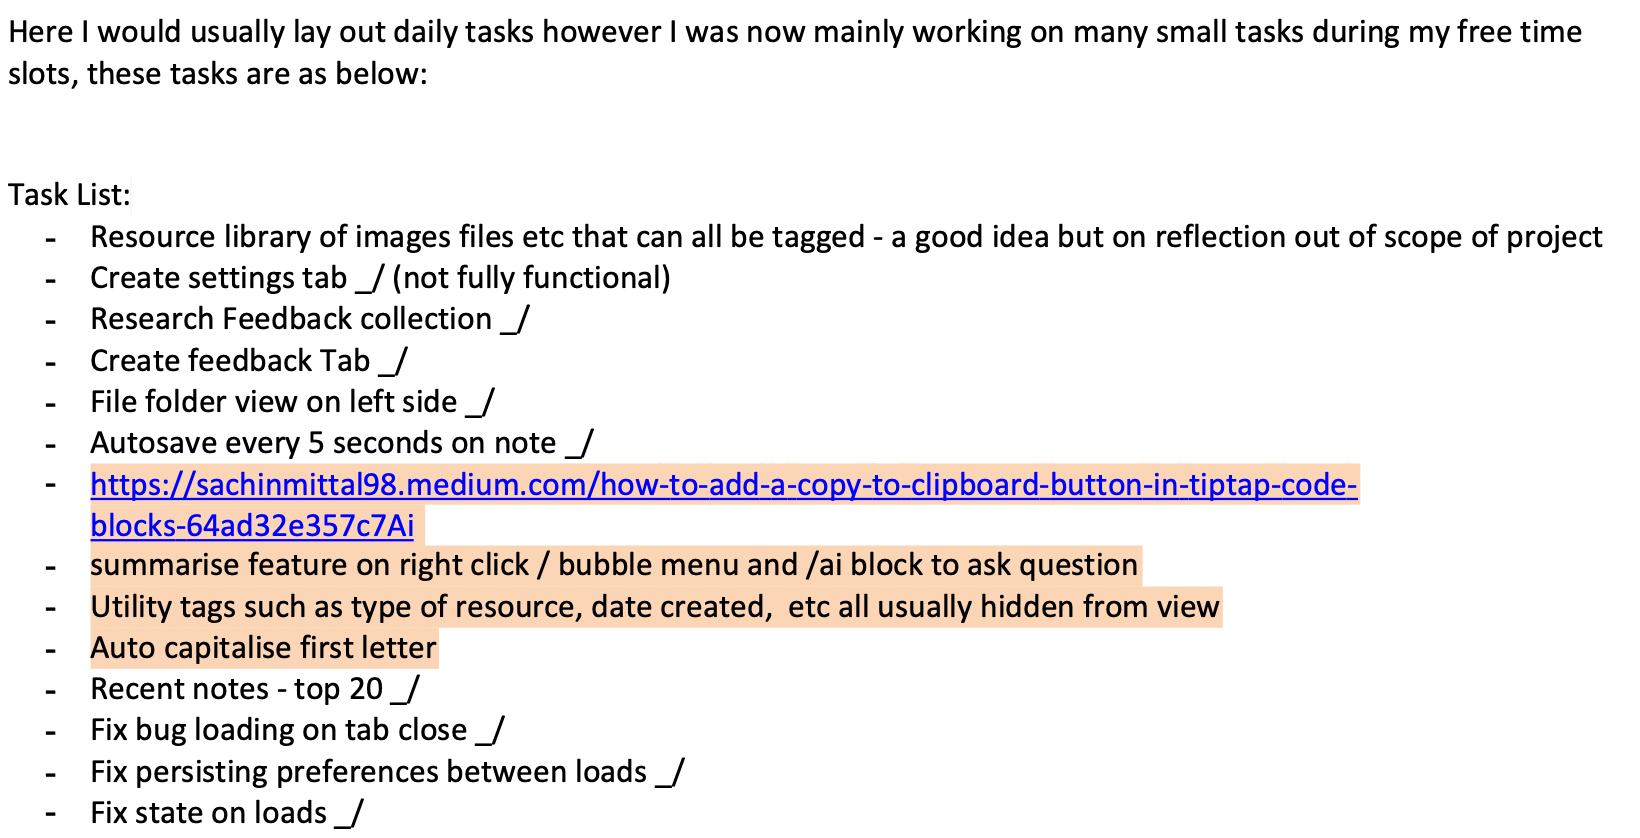
\includegraphics[width=0.8\textwidth]{SkillDevelopment/SkillsReflection/media/TodoList.png}
    \caption{Example of a task list}
\end{figure}

When I have thoughts regarding my project whilst I am out and about I use an application called TickTick to keep a running track of my thoughts and create myself mini deadlines which sync with my timelines and overall project plan.

I have found this system to be incredibly effective throughout my project, and I have been able to keep on top of my EPQ and ensure I am always working towards my goals. This has enabled me to seize the small moments in the day to grab resources online, read headlines announcing new features in technologies I am using and generally keep my mind on the project even when I am not working on it directly.


\subsection{Problem and Setback Solving:}
Throughout my project I have now come across a number of setbacks and issues whilst developing my artifact. However, due to good planning (with plenty of redundancy built in) I have never found myself behind on development. Each time I have come across a technical or theoretical (e.g. user experience) setback I immediately have spent some time problem solving but crucially limit this to a maximum of 10 minutes. I have found that stepping away from a problem and reapproaching later is an incredibly powerful tool, and I am very fortunate that my project has a number of simultaneous elements In development and I can switch between them allowing myself to think about problems in the background. I found that this method, for me personally, has been incredibly effective and has allowed me to keep a positive, productive mindset throughout my project.

\begin{figure}[H]
    \centering
    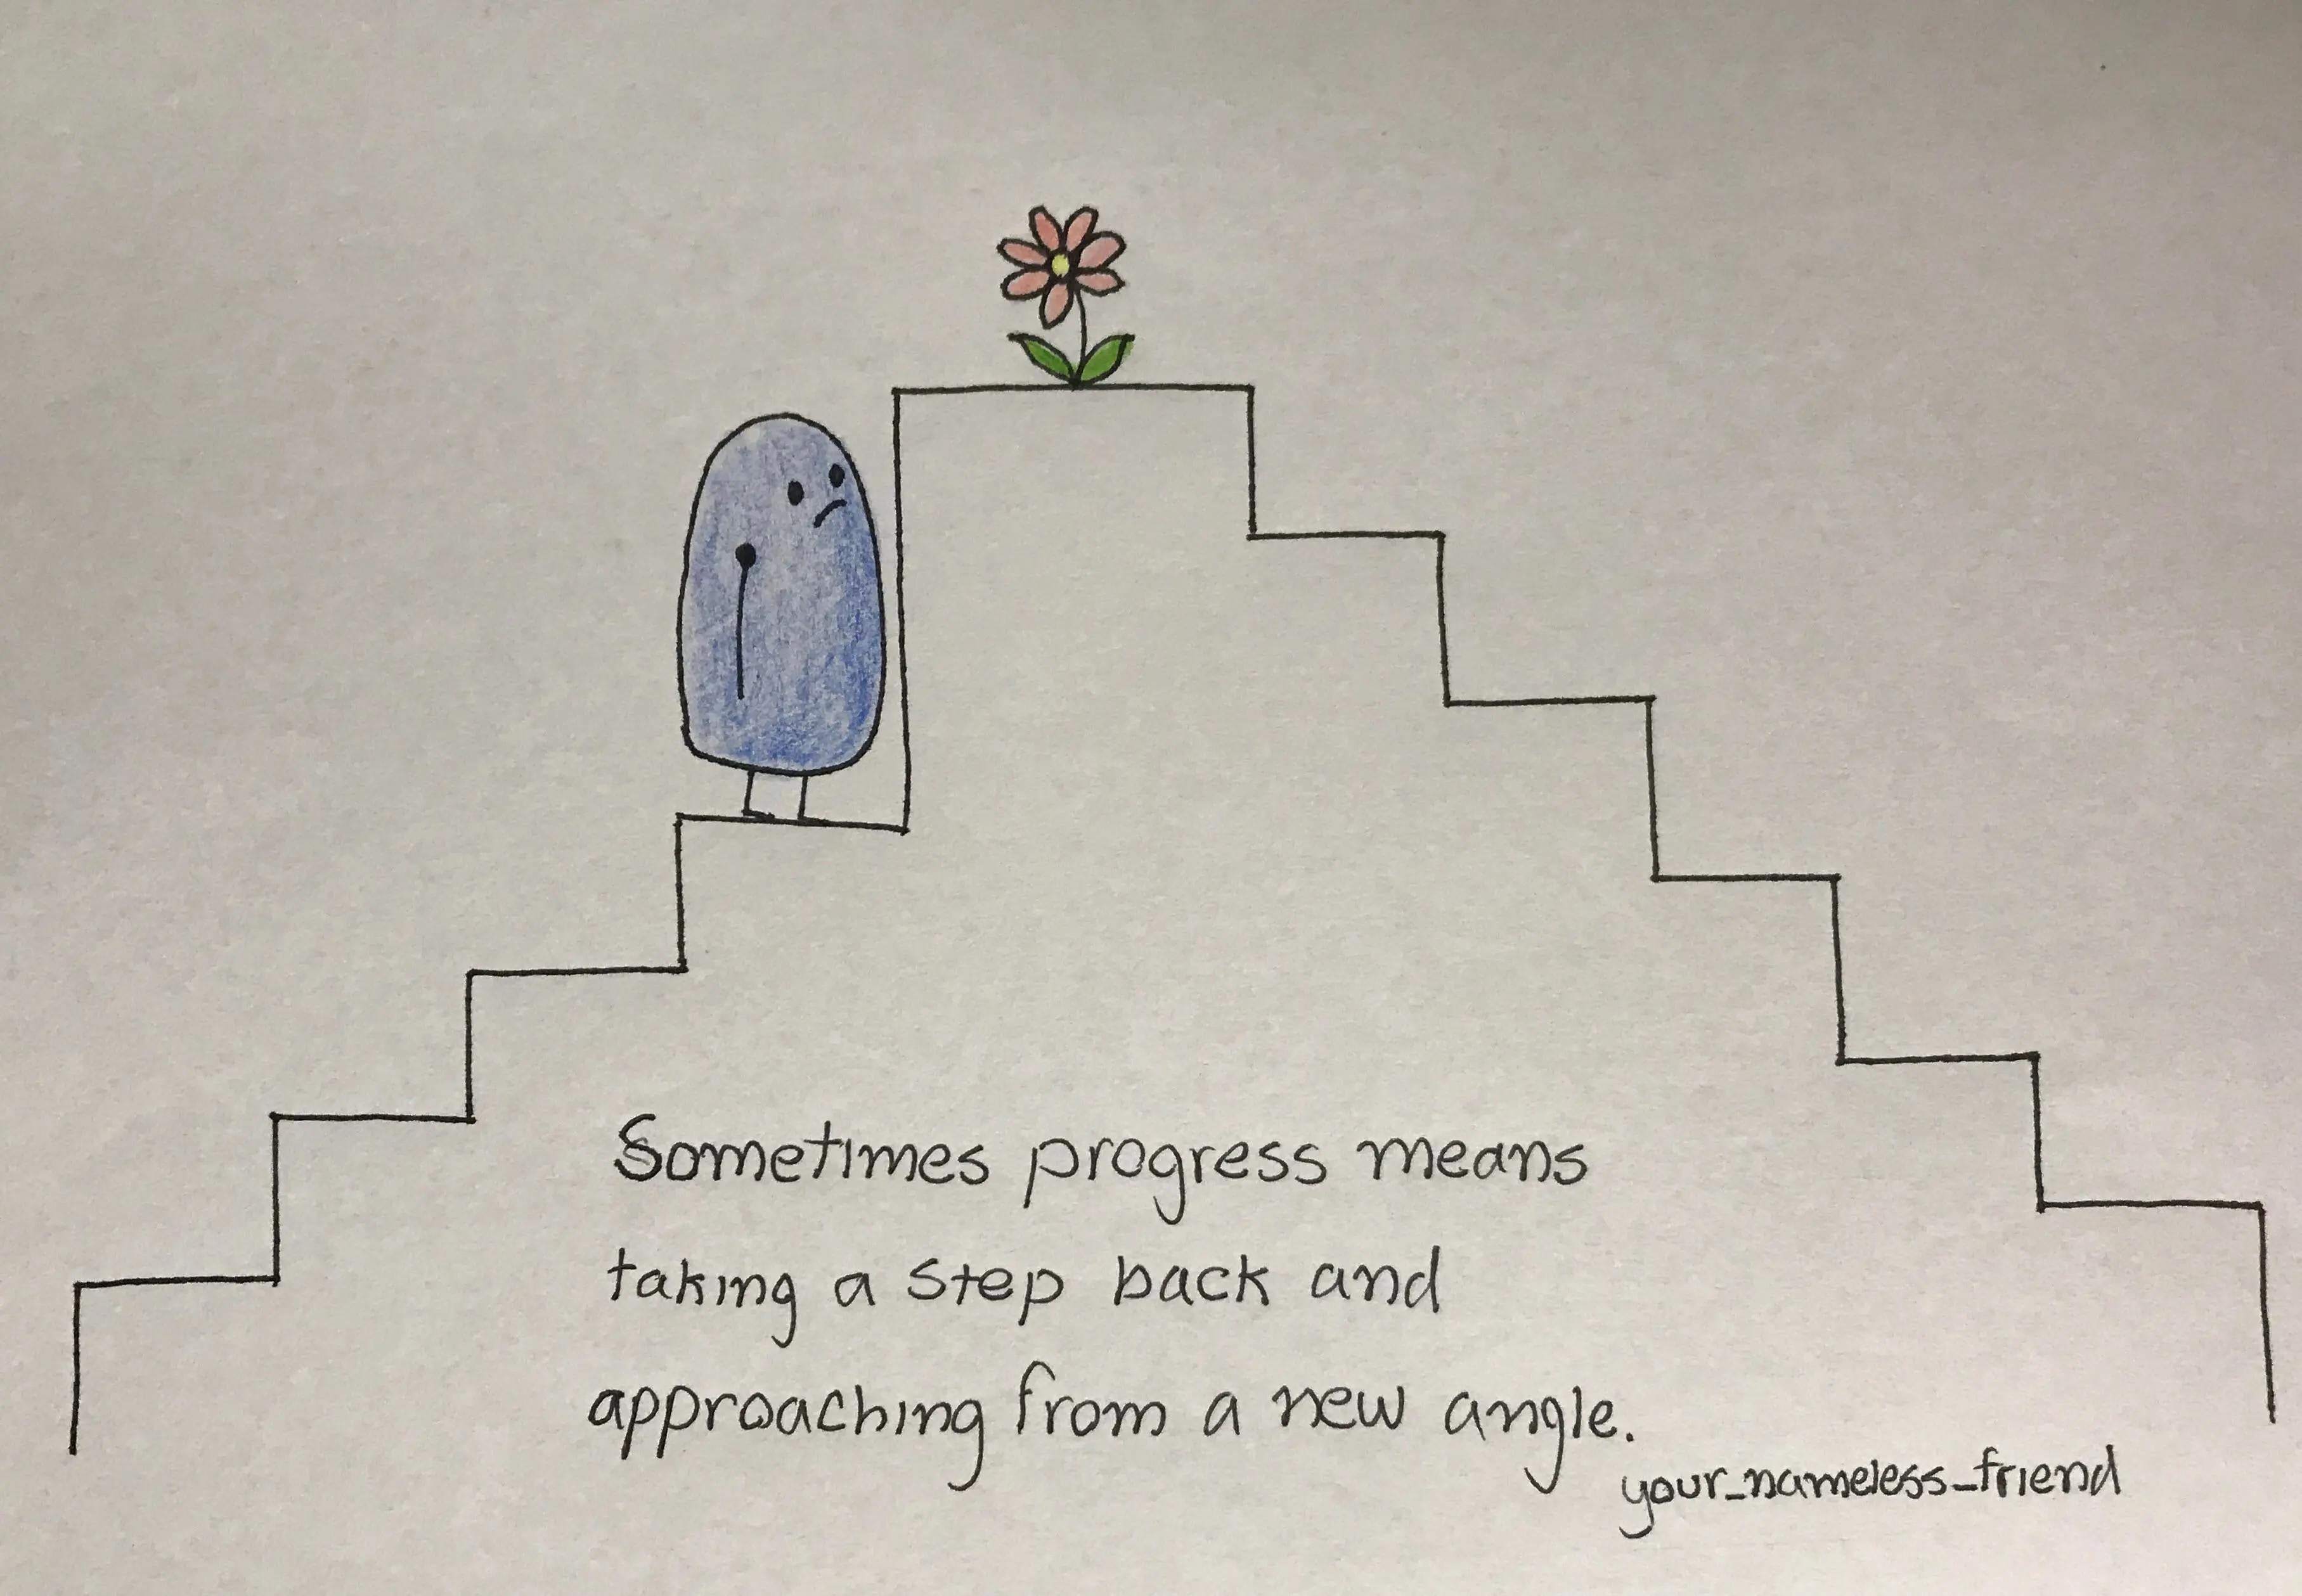
\includegraphics[width=0.8\textwidth]{SkillDevelopment/SkillsReflection/media/inspirational.png}  
    \caption{An inspirational quote I have to help me through setbacks}
\end{figure}


\subsection{User Interface Design:}
From the outset of my project, user interface(UI) design was entirely new to me-I had never designed or built anything more complex than a basic, functional interface. To build a strong foundation, I began by researching fundamental design principles, including colour theory. This early research provided me with key baseline knowledge that I continued to develop throughout the project.

To gain insight into effective UI practices, I studied a variety of popular note-taking applications. I analysed their design choices, aesthetics, and how they presented similar features in different ways. This comparative analysis helped me understand industry standards and user expectations, allowing me to build on successful ideas while also identifying areas for improvement.

With some design ideas forming, I turned to Figma to begin prototyping. Learning to use a professional design tool significantly boosted both my creativity and efficiency. It gave me a deeper appreciation for the mindset and processes used by professionals in the field, and allowed me to rapidly experiment with interface concepts.

I also involved peers and friends in my design process to gather feedback on key UX elements, such as tab switching and branding. Although opinions varied, I was able to identify common themes in what users considered a “good” experience, which helped shape my final design direction.
\begin{figure}[H]
    \centering
    \begin{tabular}{cc}
        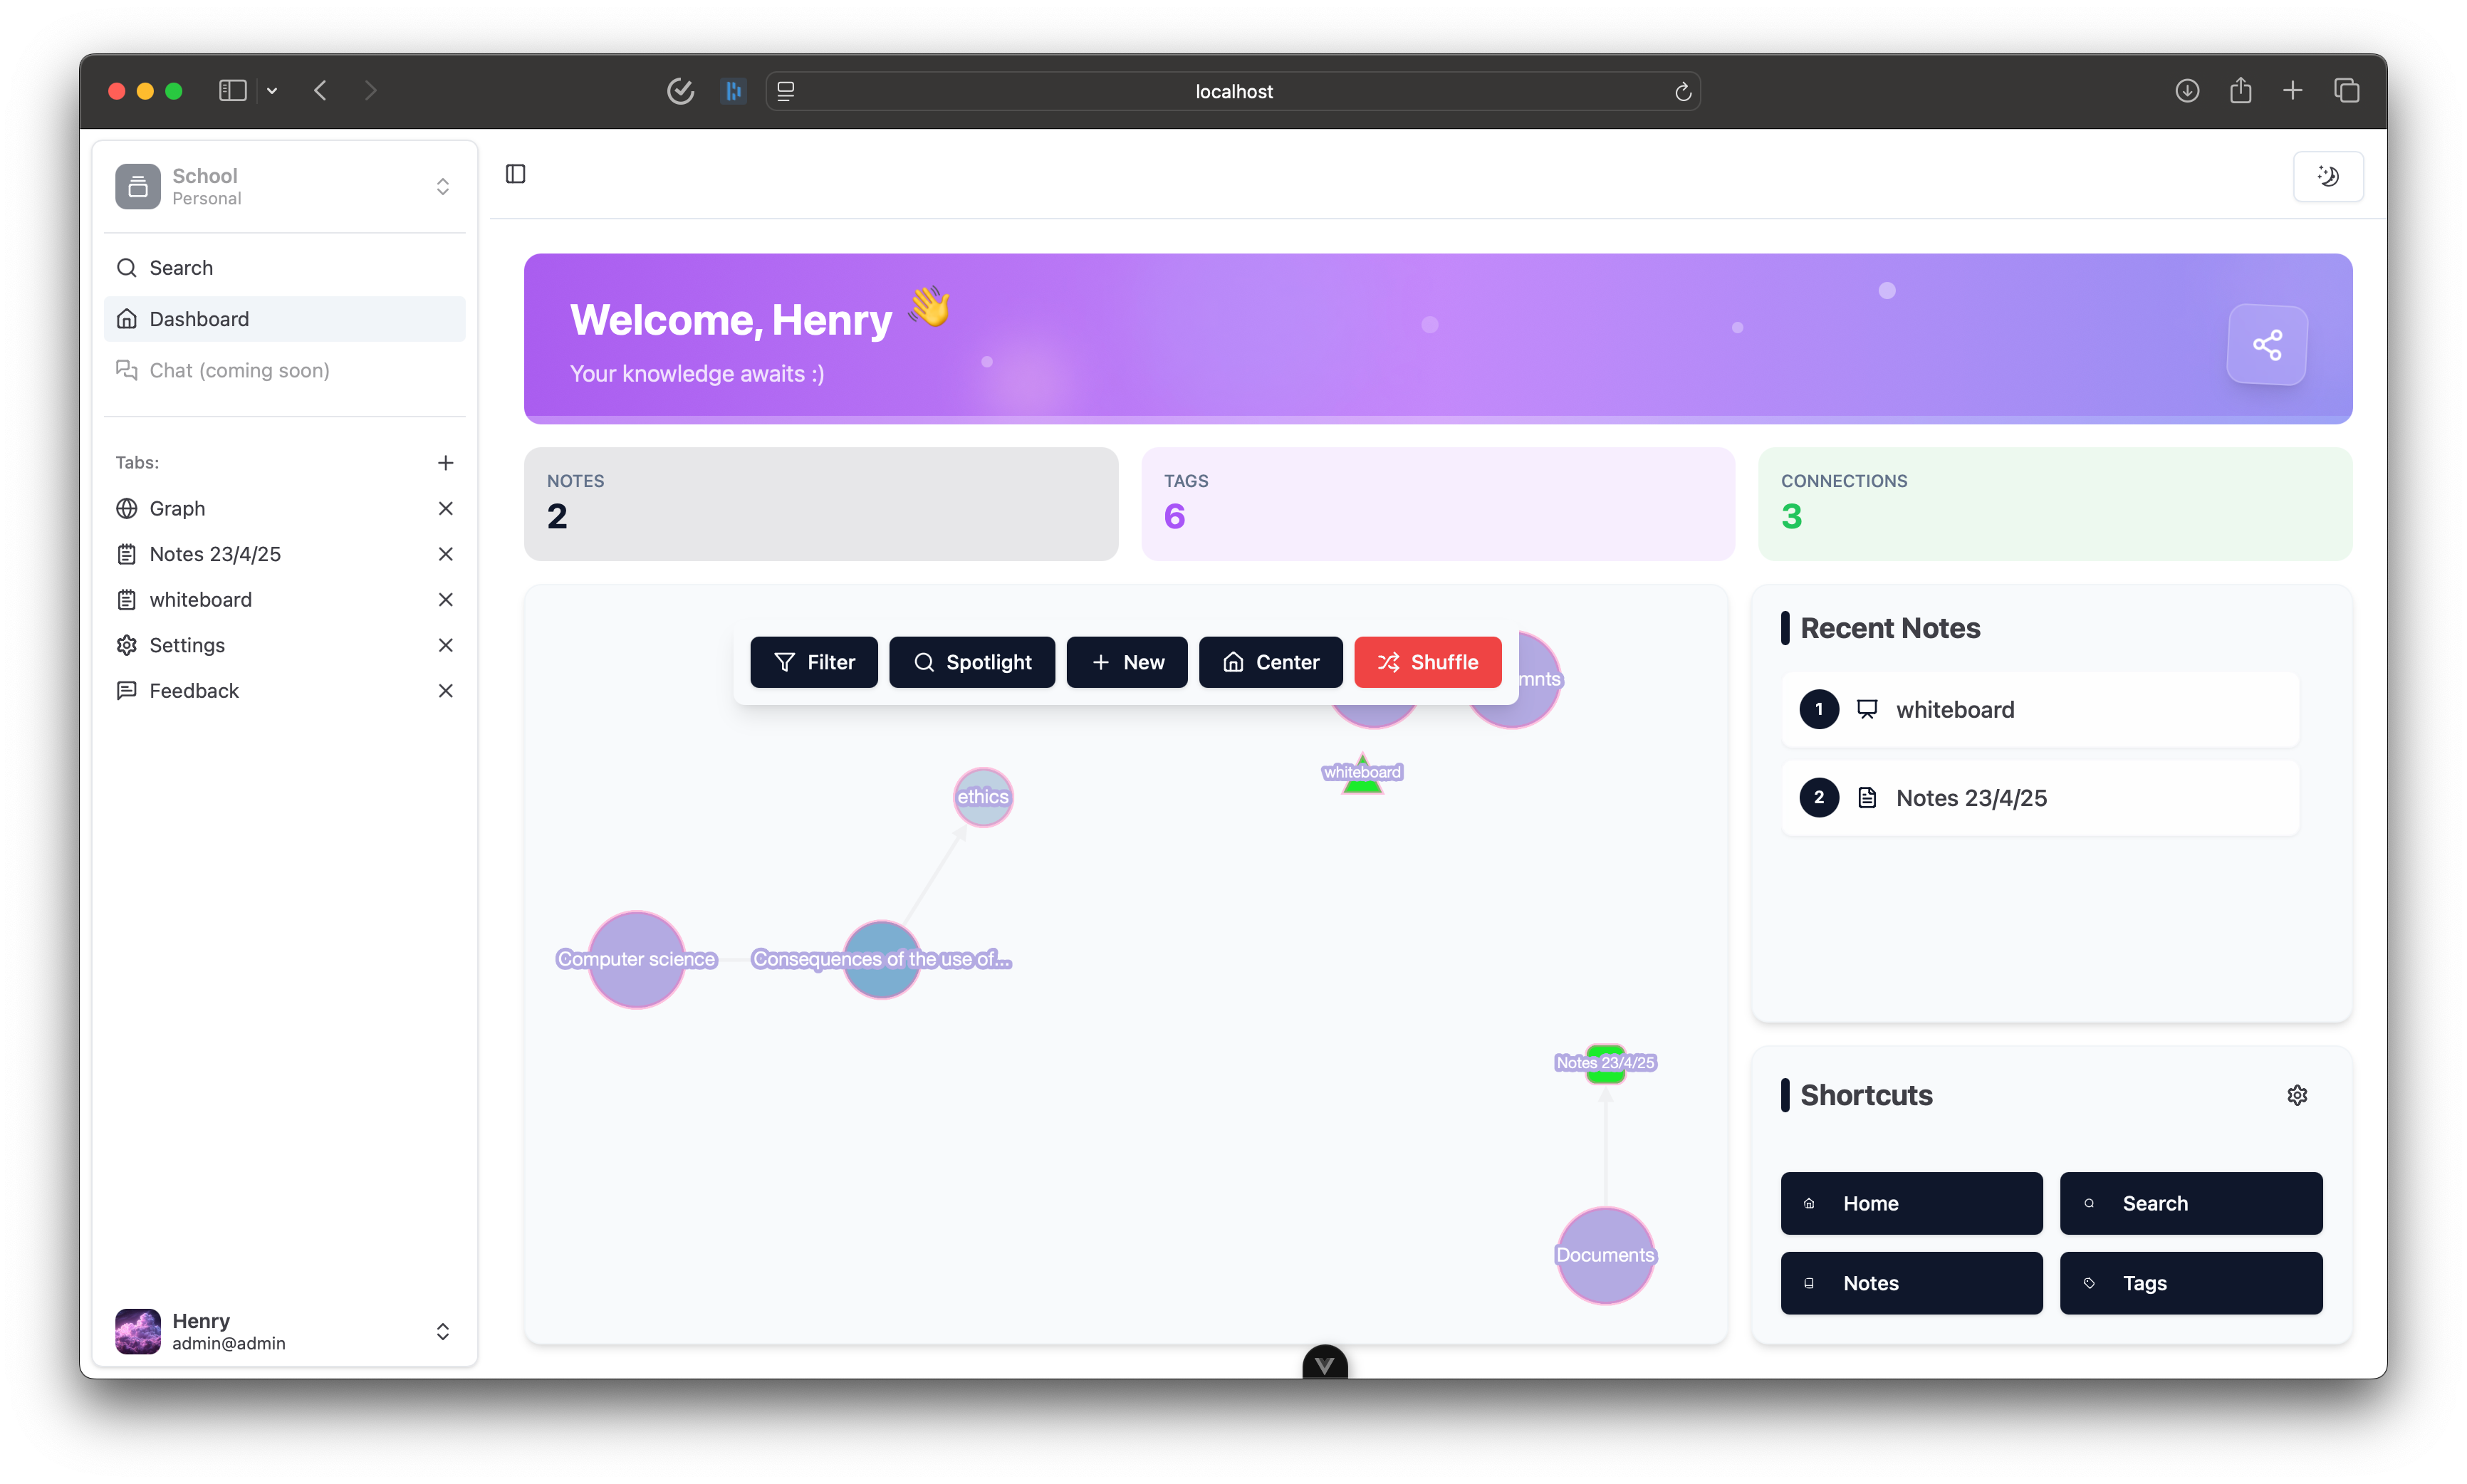
\includegraphics[width=0.45\textwidth]{SkillDevelopment/SkillsReflection/media/ui1.png} &
        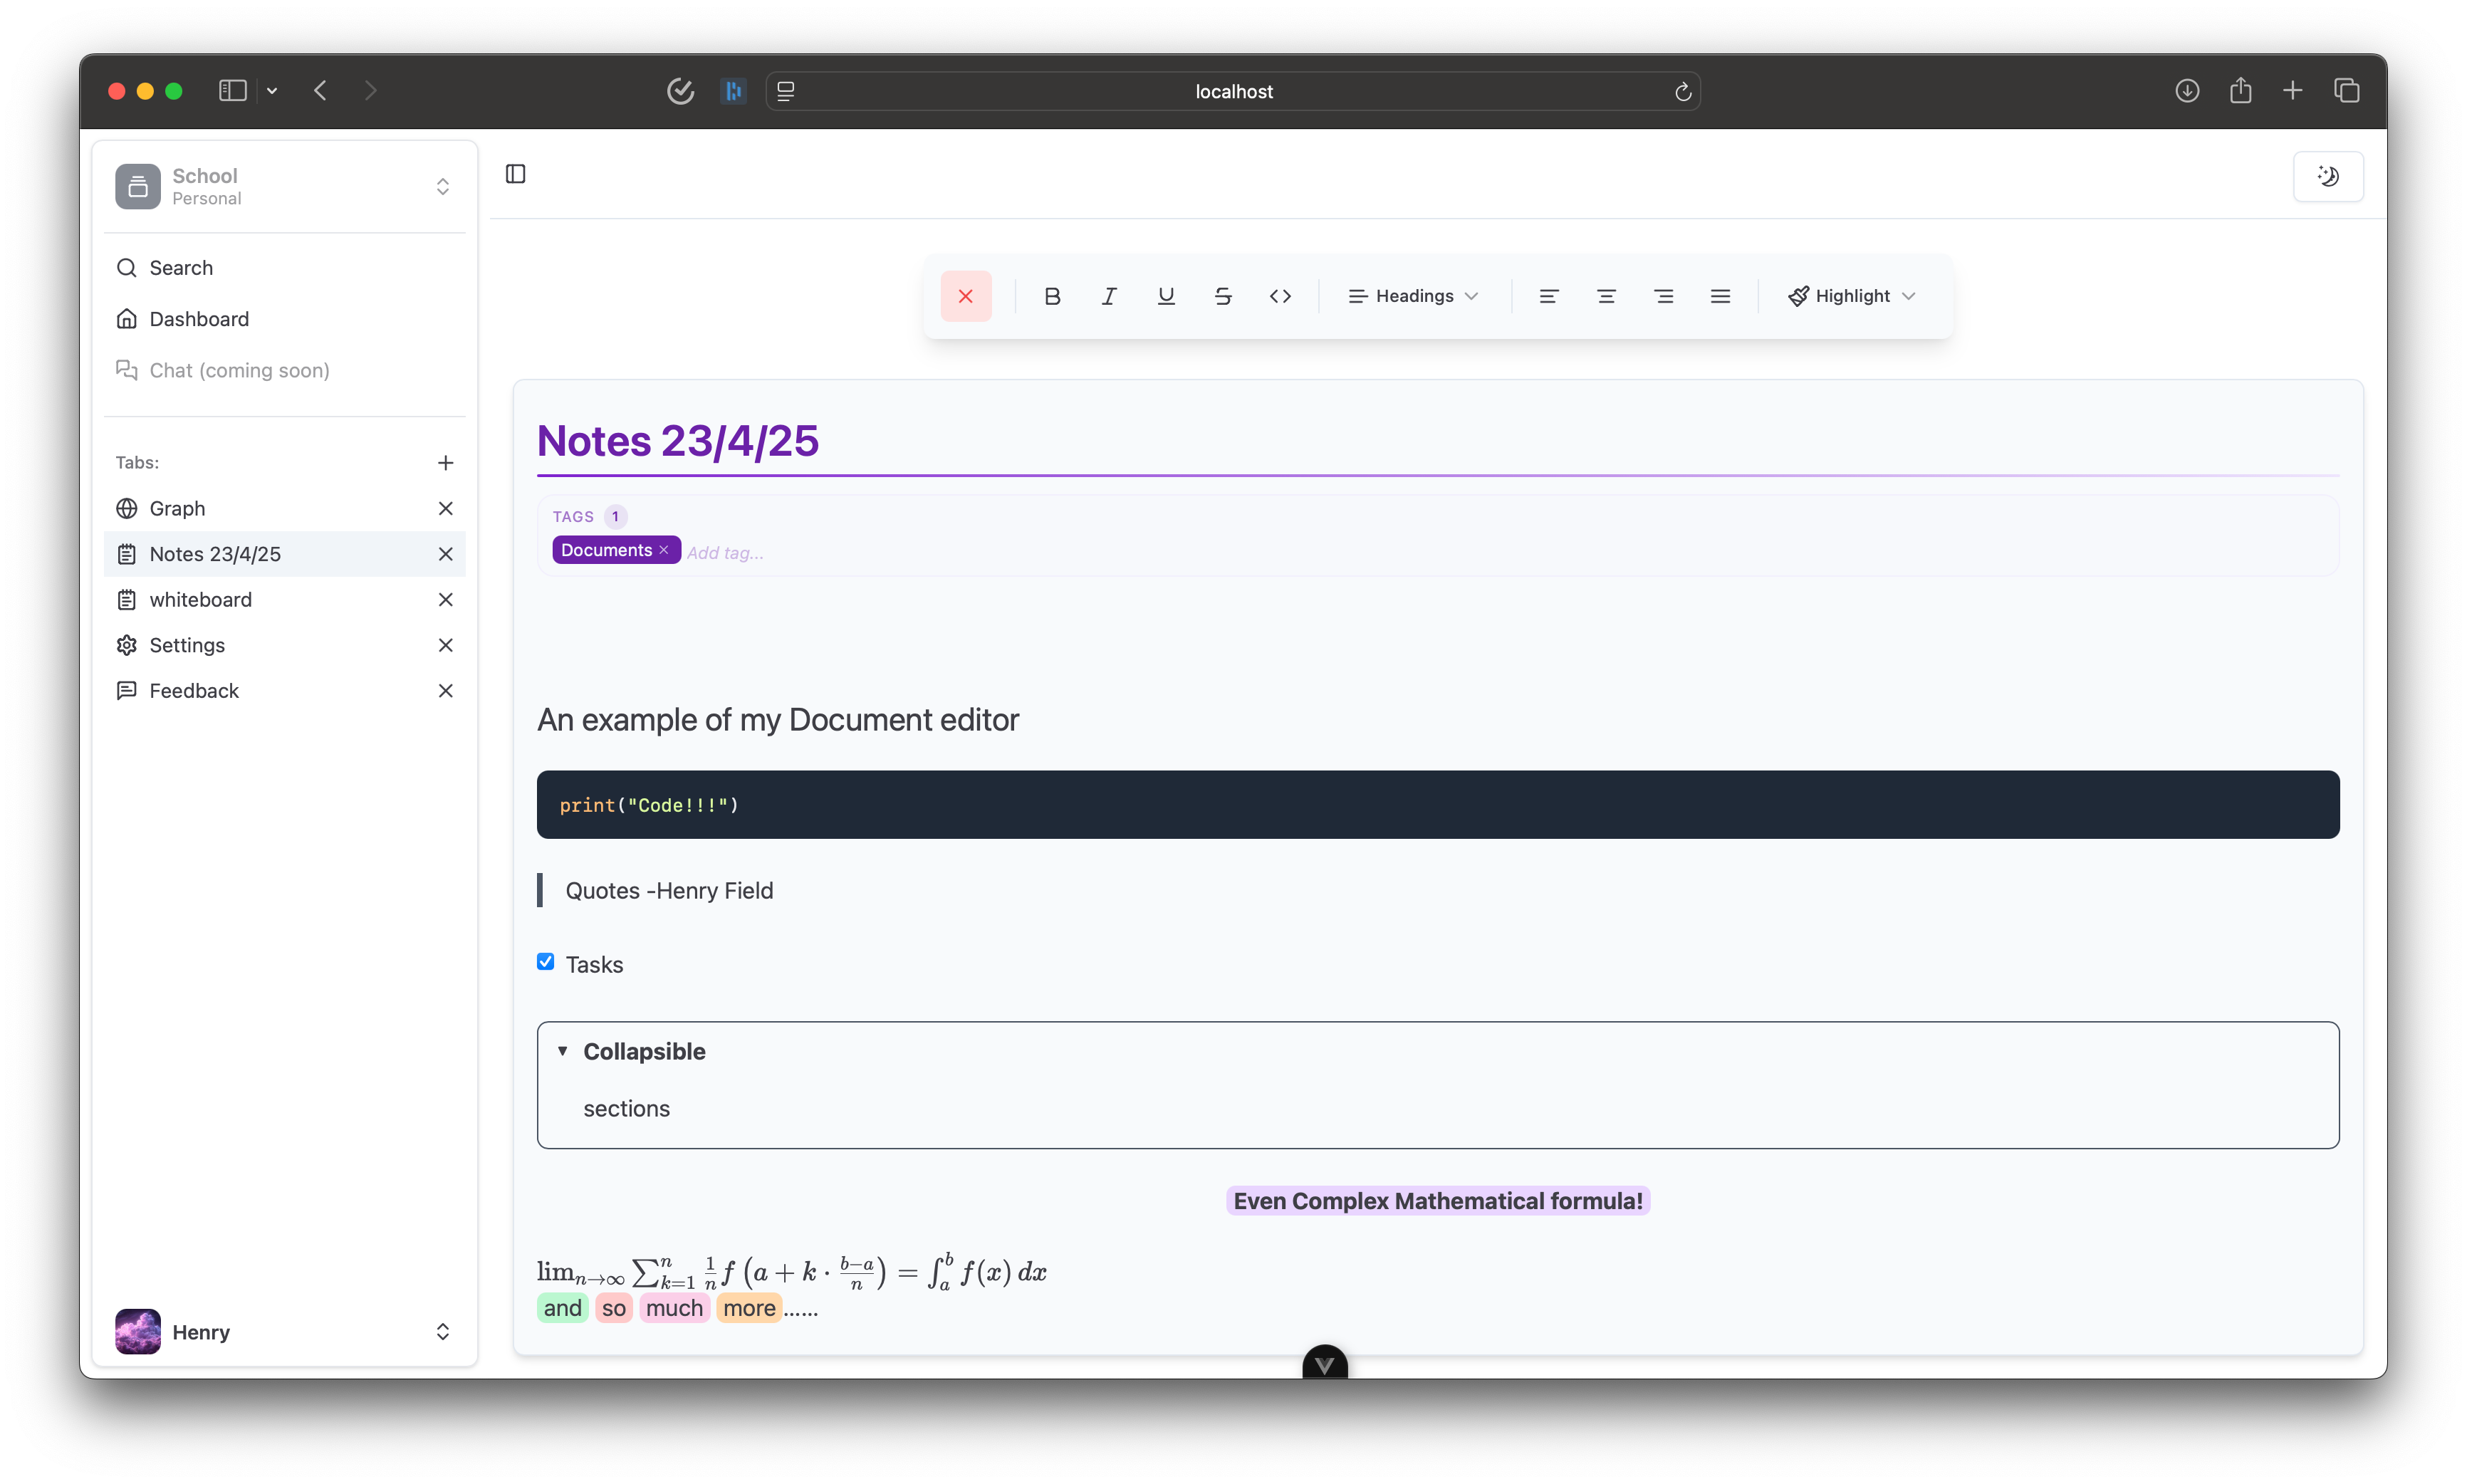
\includegraphics[width=0.45\textwidth]{SkillDevelopment/SkillsReflection/media/ui2.png} \\
        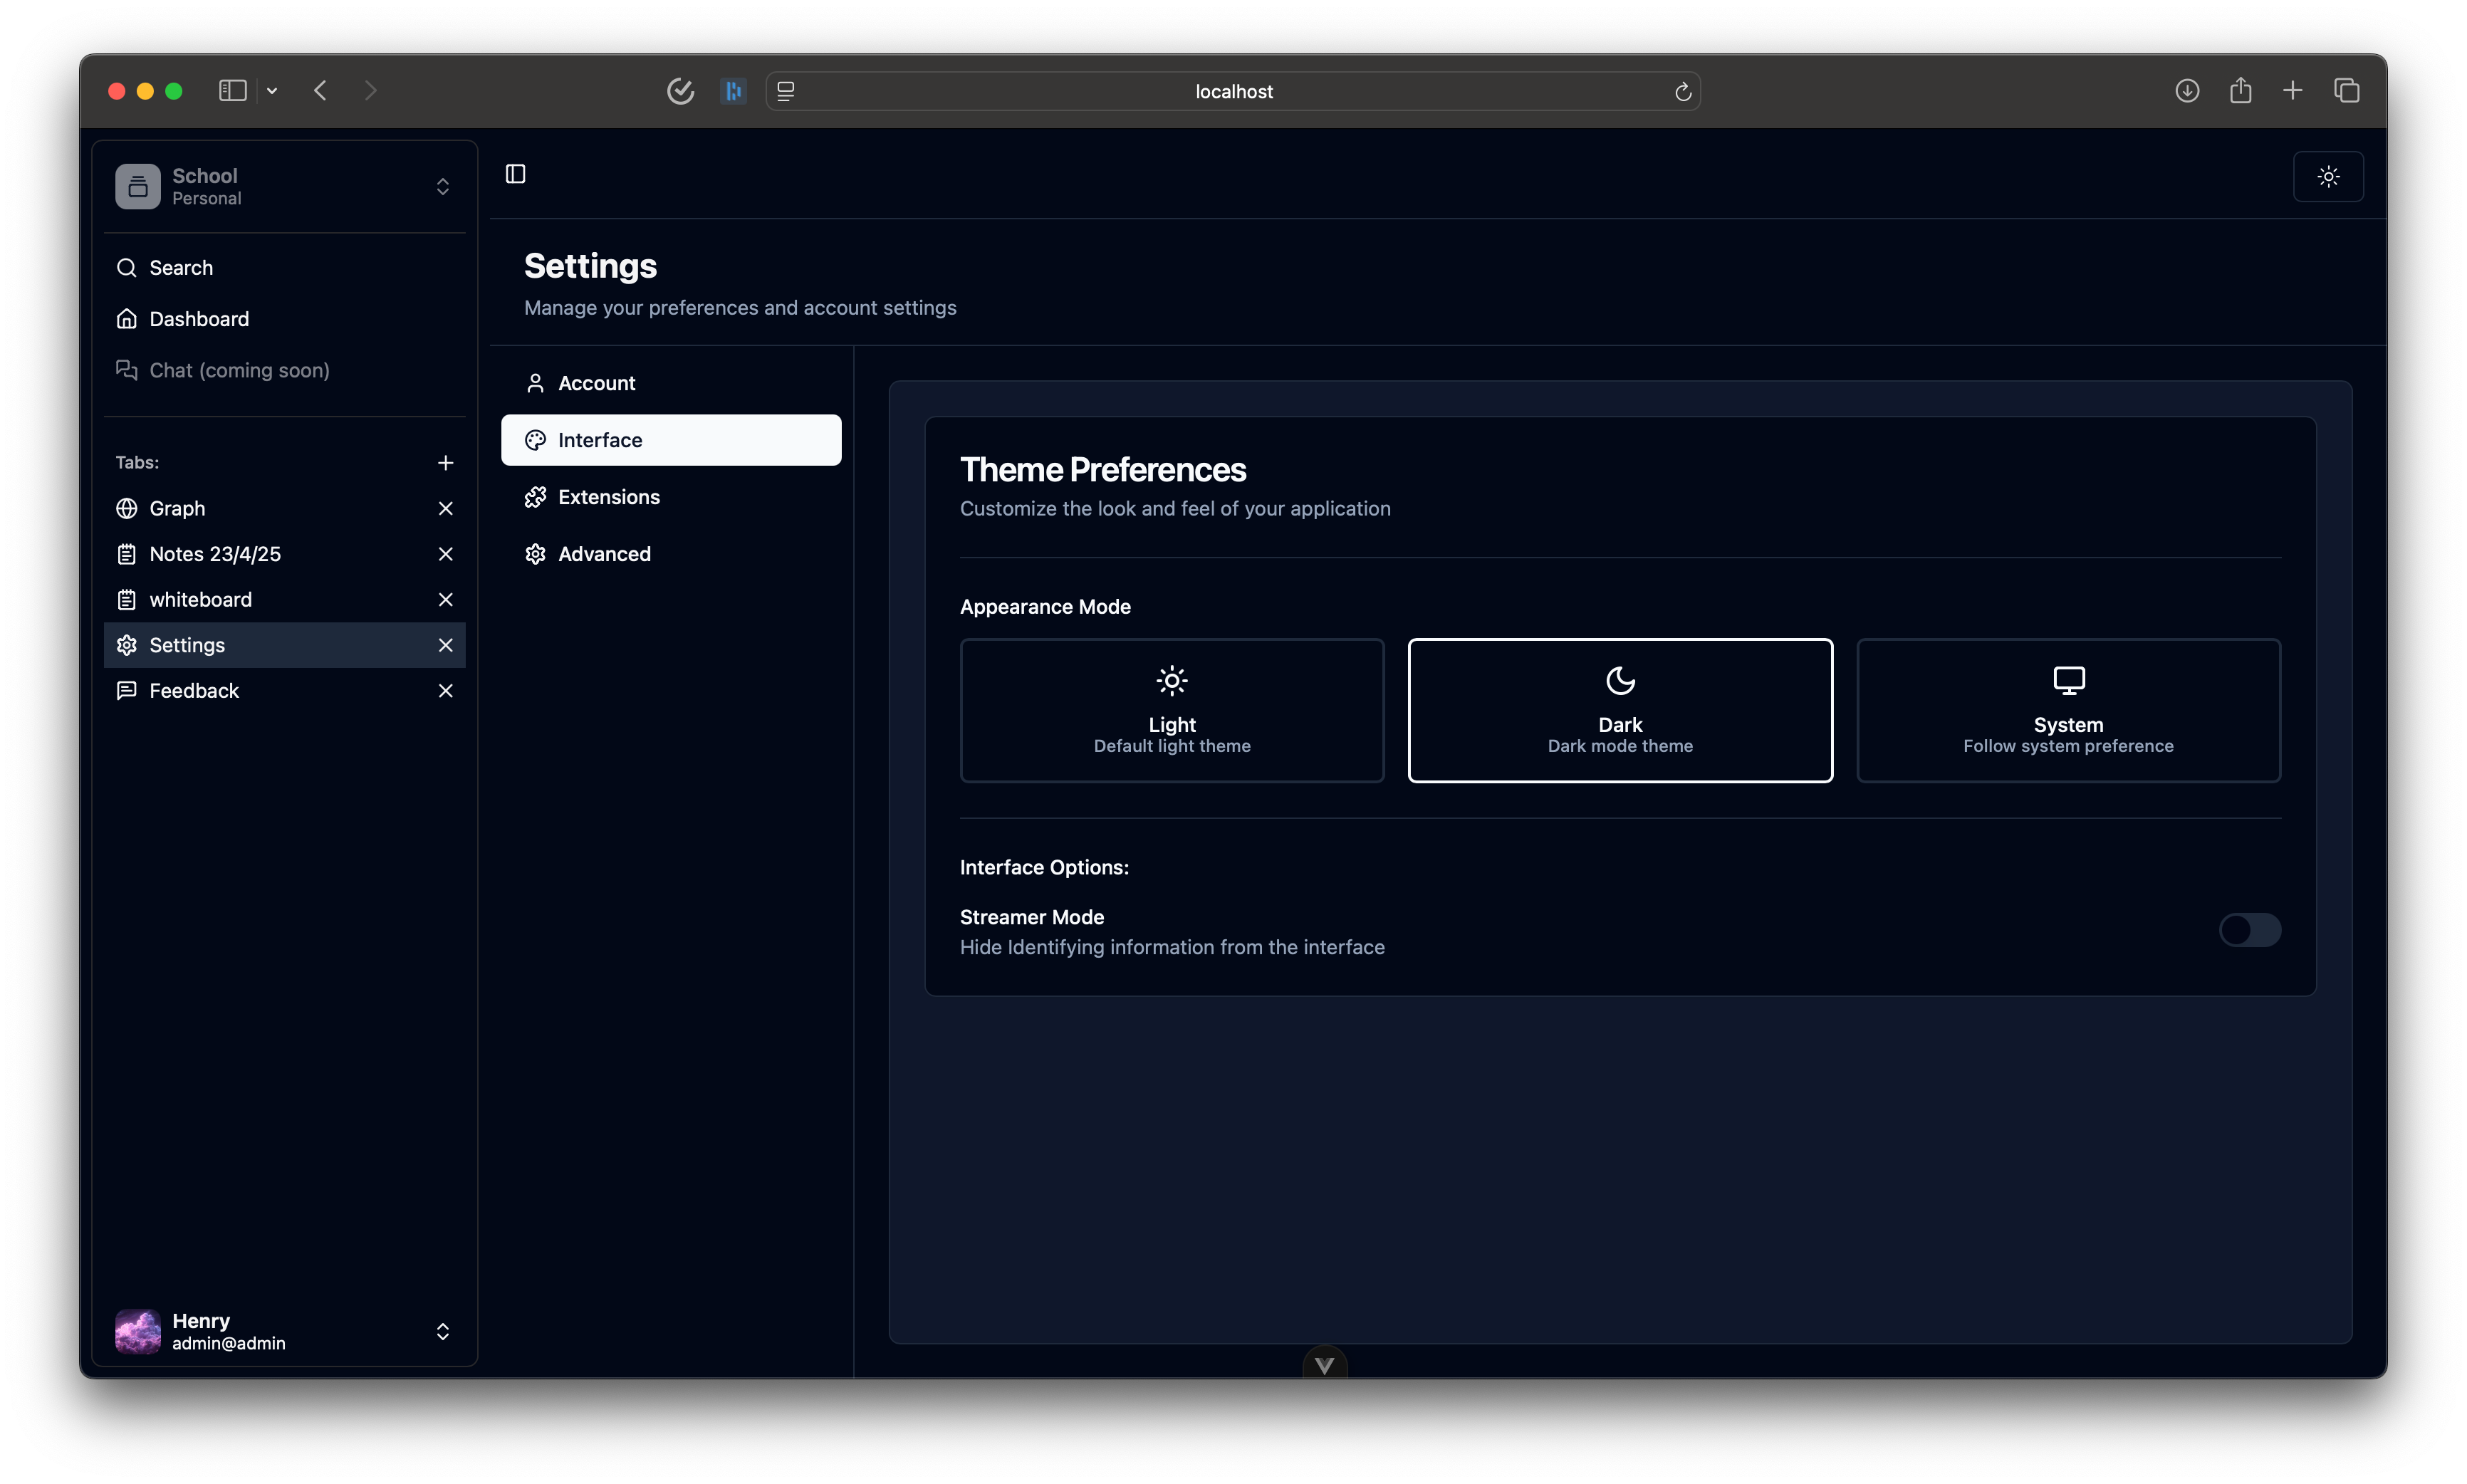
\includegraphics[width=0.45\textwidth]{SkillDevelopment/SkillsReflection/media/ui3.png} &
        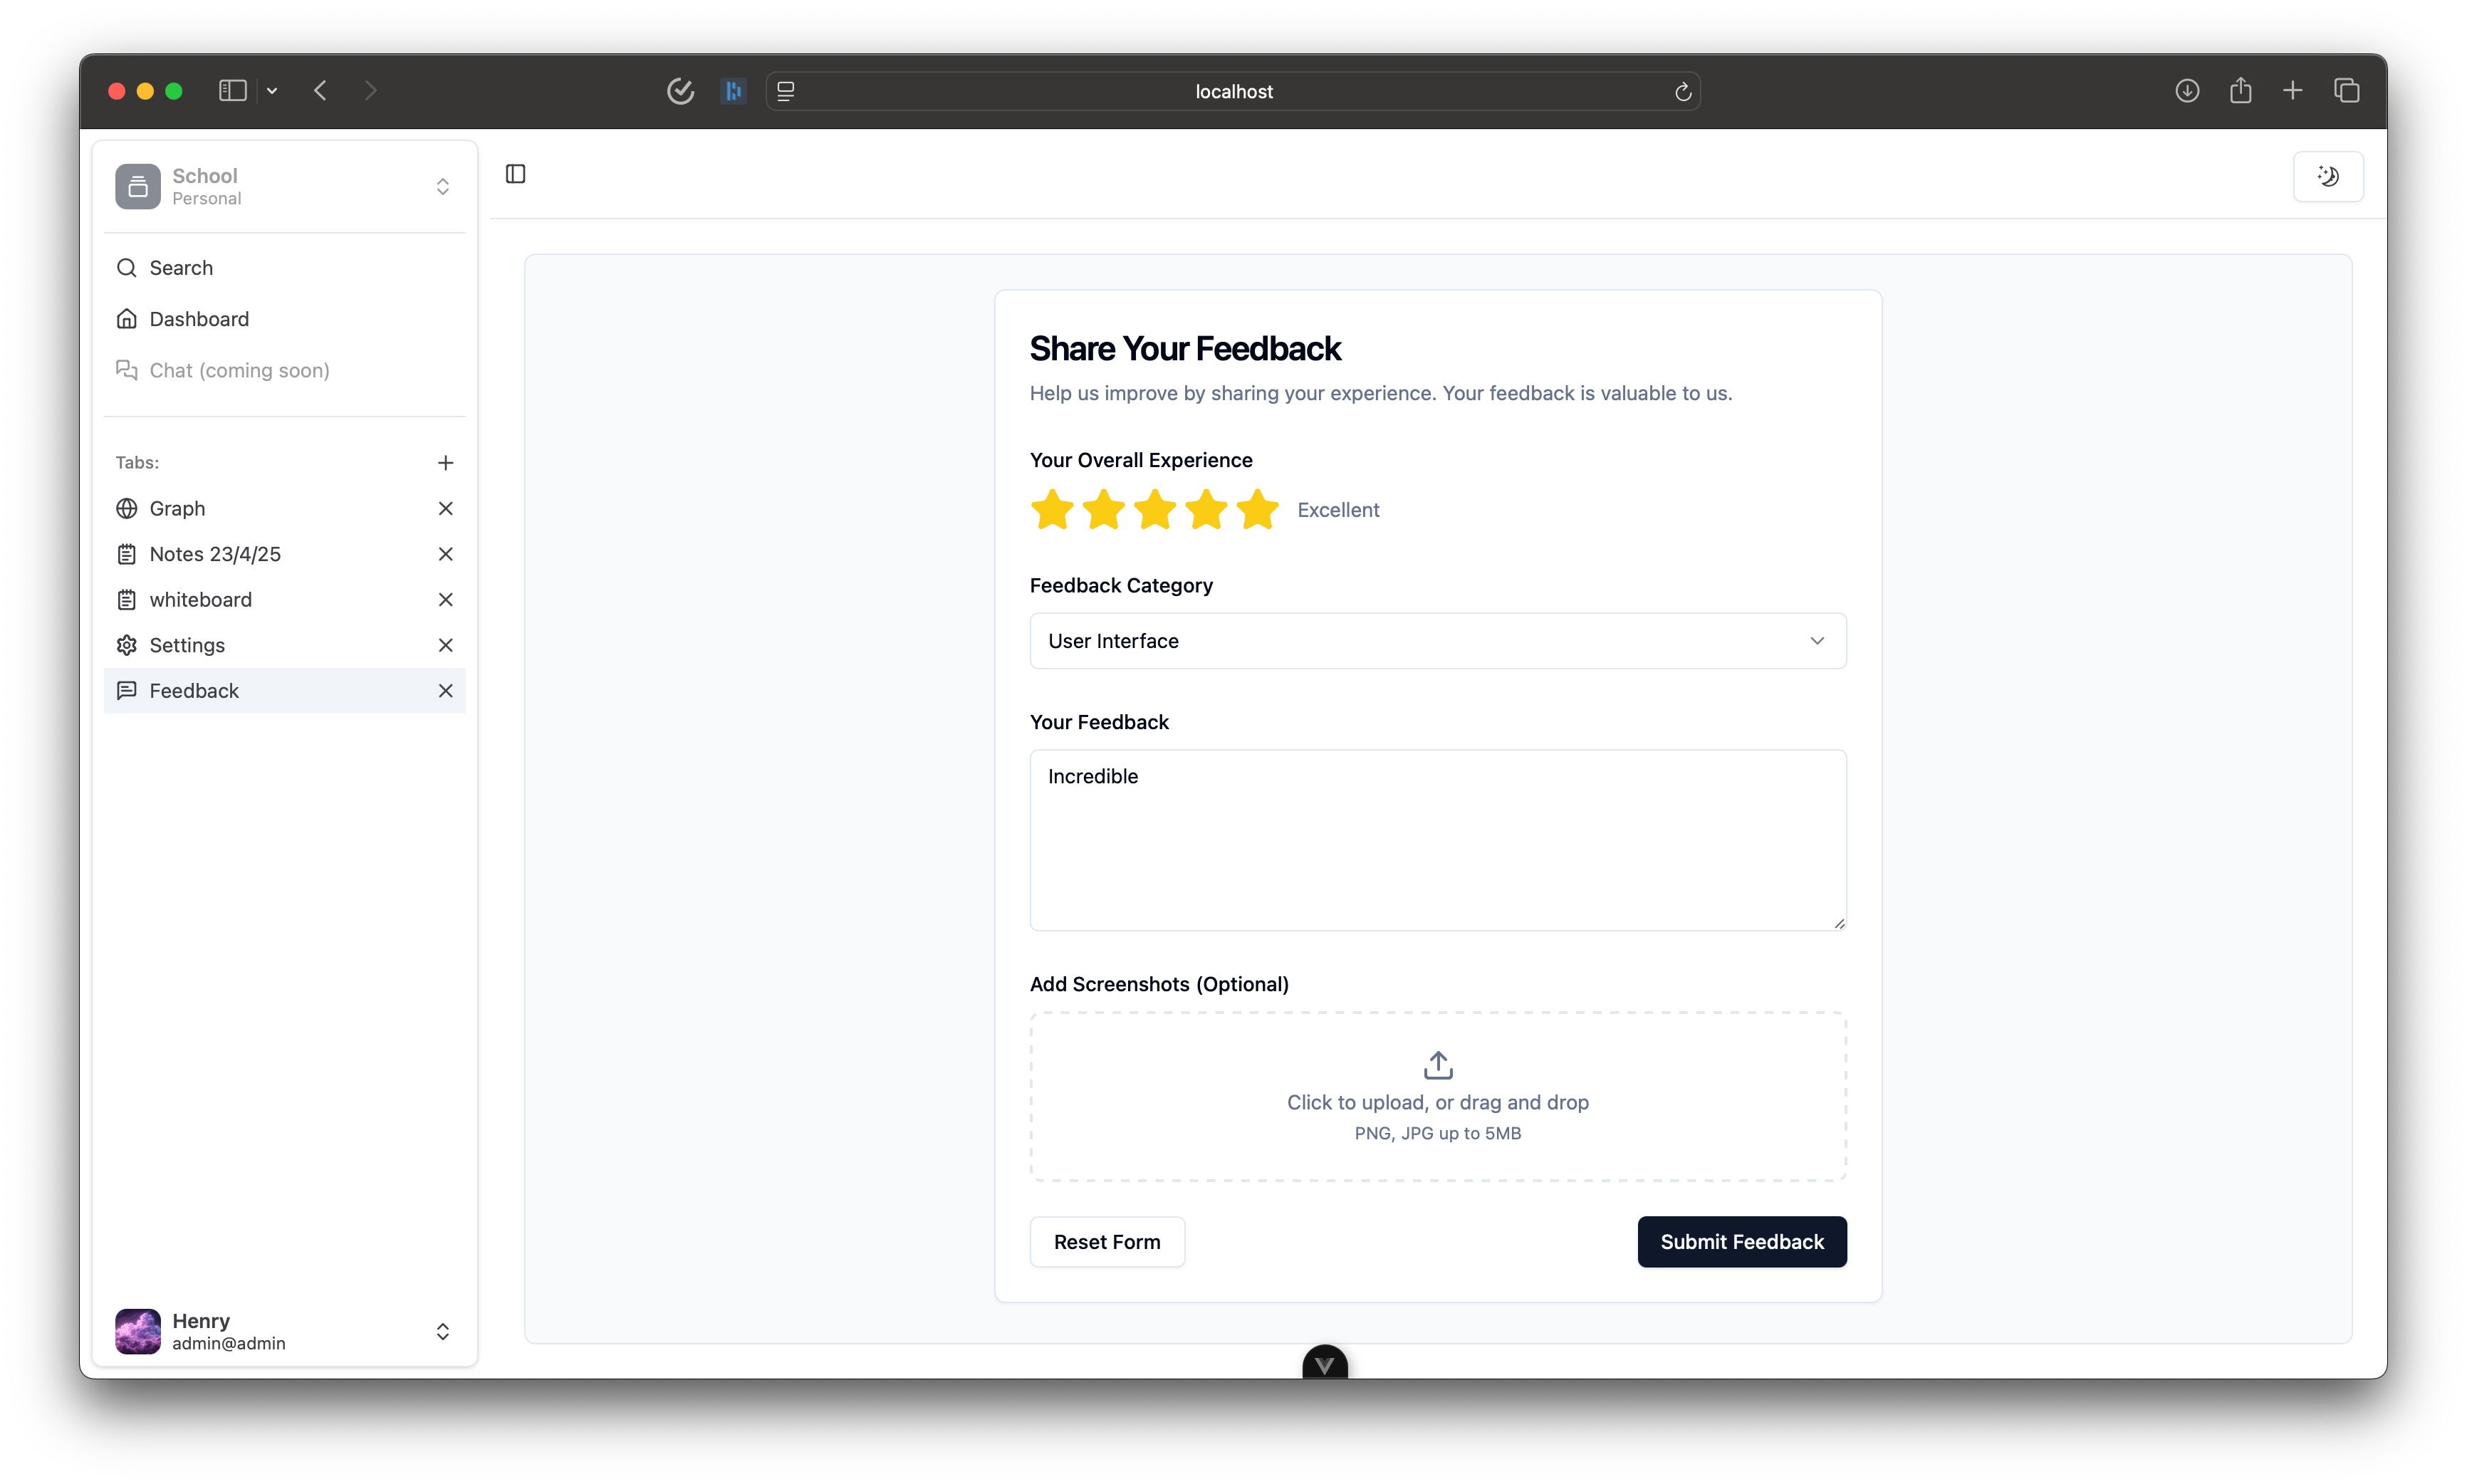
\includegraphics[width=0.45\textwidth]{SkillDevelopment/SkillsReflection/media/ui4.png} \\
    \end{tabular}
    \caption{Examples of user interface designs}
\end{figure}

\subsection{User Experience Design:}
As my project progressed, I began to understand that user experience (UX) design is much more than simply making something “look nice.” It is about creating a flow that feels natural, reduces friction, and allows the user to focus on their task (producing detailed, efficient notes) rather than the tool. This was especially important for my project since note-taking applications should aid learning, not distract from it. I researched common UX principles and best practices, such as accessibility guidelines, and began to apply these concepts to my designs.

A huge part of UX is understanding the user's journey through an application. I mapped out typical user flows for key tasks, such as creating and organising notes, to ensure that each step was intuitive and efficient. This process highlighted potential pain points and areas where I could streamline interactions.

To further refine my UX skills, I studied established applications to see how they handled similar challenges. I paid close attention to how they balanced functionality with simplicity, and how they guided users through complex tasks without overwhelming them. By evaluating both the strengths and weaknesses of these applications, I was able to extract valuable lessons that informed my own design decisions.

To put these principles into practice, I tested many versions of my prototype with peers, observing how they interacted with the system. Their feedback revealed that even small choices, such as the placement of menus or the speed of animations, had a noticeable effect on usability. This iterative process taught me to place users at the centre of every design decision, and I found myself increasingly confident in applying UX thinking to technical decisions.

\subsection{Graphic Design:}
Before starting this project, I had very limited experience with graphic design, and most of my previous work had been purely functional rather than aesthetic. However, as I began to shape the visual identity of my artefact, I realised how essential good design is for building credibility and creating a professional-looking product. I studied aspects of design such as typography, colour palettes, and visual hierarchy, ensuring that my choices aligned with my branding and target audience.

Using tools like Figma and Illustrator allowed me to experiment with different layouts and styles quickly. For example, I iterated through several Welcome Page designs before settling on one that captured both the “neuron” and “notetaking” aspects of my product. This process showed me how design can communicate meaning subconsciously, shaping how users perceive the software even before they begin interacting with it. I developed a stronger eye for detail and gained confidence in blending creativity with consistency.

\begin{figure}[H]
    \centering
    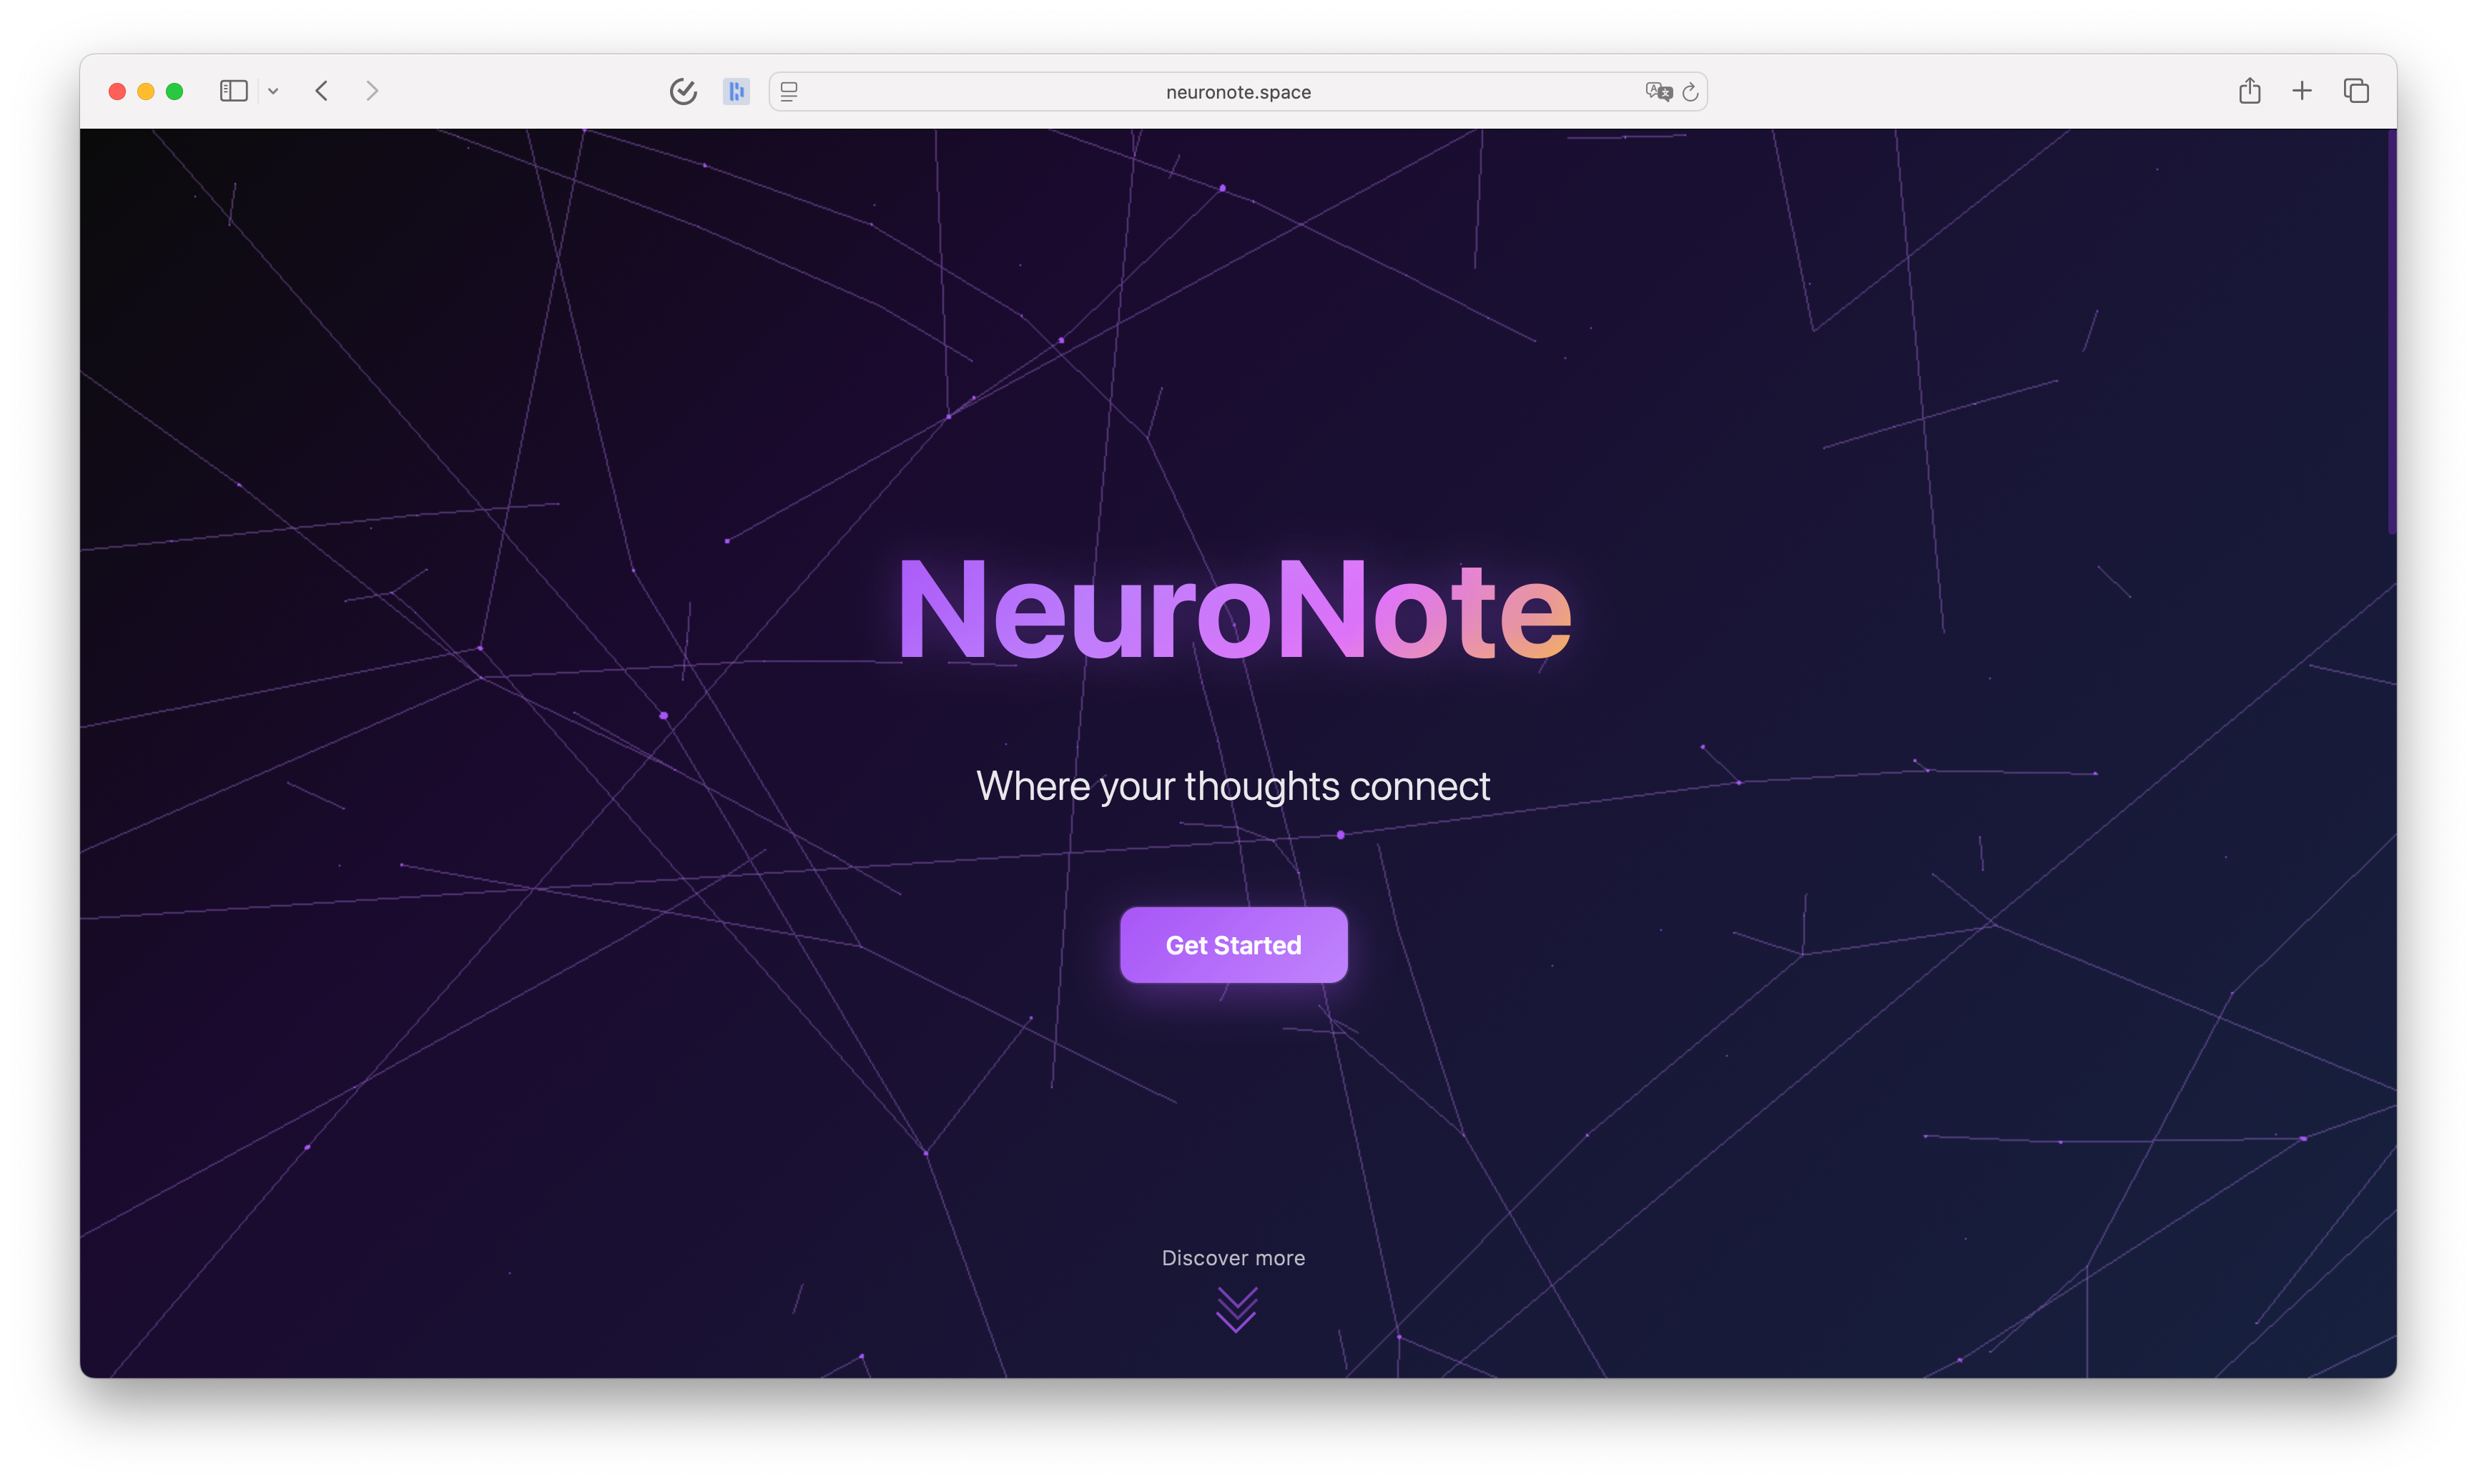
\includegraphics[width=0.8\textwidth]{SkillDevelopment/SkillsReflection/media/welcomePage.png}
    \caption{My final animated welcome page design}
\end{figure}

\subsection{Product Naming and Theming:}

Choosing a name and colour theme for my project was more challenging than I initially expected. A product's name is not only a label but also part of its identity, influencing how users relate to it and whether they perceive it as professional and trustworthy. After brainstorming a wide range of possibilities, I settled on NeuroNote. The name reflects the psychological inspiration behind the project and its function, while remaining short, memorable, and practical as a brand.

Developing the theme around the name allowed me to unify the project's identity. I drew inspiration from neural networks and brain imagery, incorporating subtle references to connections and learning throughout the UI and branding. Additionally, I completed some research on the subconscious impact colour has on our perception of trust and confidence,  using colours which inspired these positive traits is just one more tool I have to give my users a positive experience before ever even using the project. This theming process taught me that branding is not just a superficial detail but a way to align all parts of a product - from its interface to its marketing, into a coherent and viable asset. 

\subsection{Typing:}

Although typing is an everyday skill, working on my EPQ made me appreciate it in a new way. Writing long reports, coding scripts, and documenting progress all required accuracy and speed. By spending so much time in development environments and word processors, I naturally improved my typing fluency, particularly when switching between natural language and technical code.

To further improve my typing speed I completed the KAZ Learn to type course which helped me increase my speed/accuracy on their 'complex passage test' from 53WPM/93\% accuracy to 78WPM/99\% accuracy - a significant improvement.

I also began adopting keyboard shortcuts and command-line tools to speed up my workflow. For example, within coding I used shortcuts for quickly navigating between files, and within research I used text expansion tools to format notes efficiently and precise "regex" search tools to find the content i needed more. This small but important skill became a foundation for productivity, reminding me that even basic abilities can develop significantly when applied intensively over a long-term project.
\subsection{Database Management:}
Before my EPQ, databases were a concept I had only encountered briefly whilst trying to store data long-term within projects. Developing NeuroNote required me to work hands-on with industry standard systems, specifically PostgreSQL, which introduced me to data structures, query optimisation, and technicalities surrounding the security and uptime of a 'professional' data store. Learning how to model notes and user accounts in a database gave me practical insight into how data-driven applications are built.

One of the main challenges I faced was designing the database to be flexible but efficient. I experimented with different structures for storing handwritten and typed notes, weighing up trade-offs between performance and scalability. This taught me the importance of planning databases carefully before implementation. By the end of the project, I felt far more confident in managing structured information and recognised database skills as essential to almost any modern software project.

\begin{figure}[H]
    \centering
    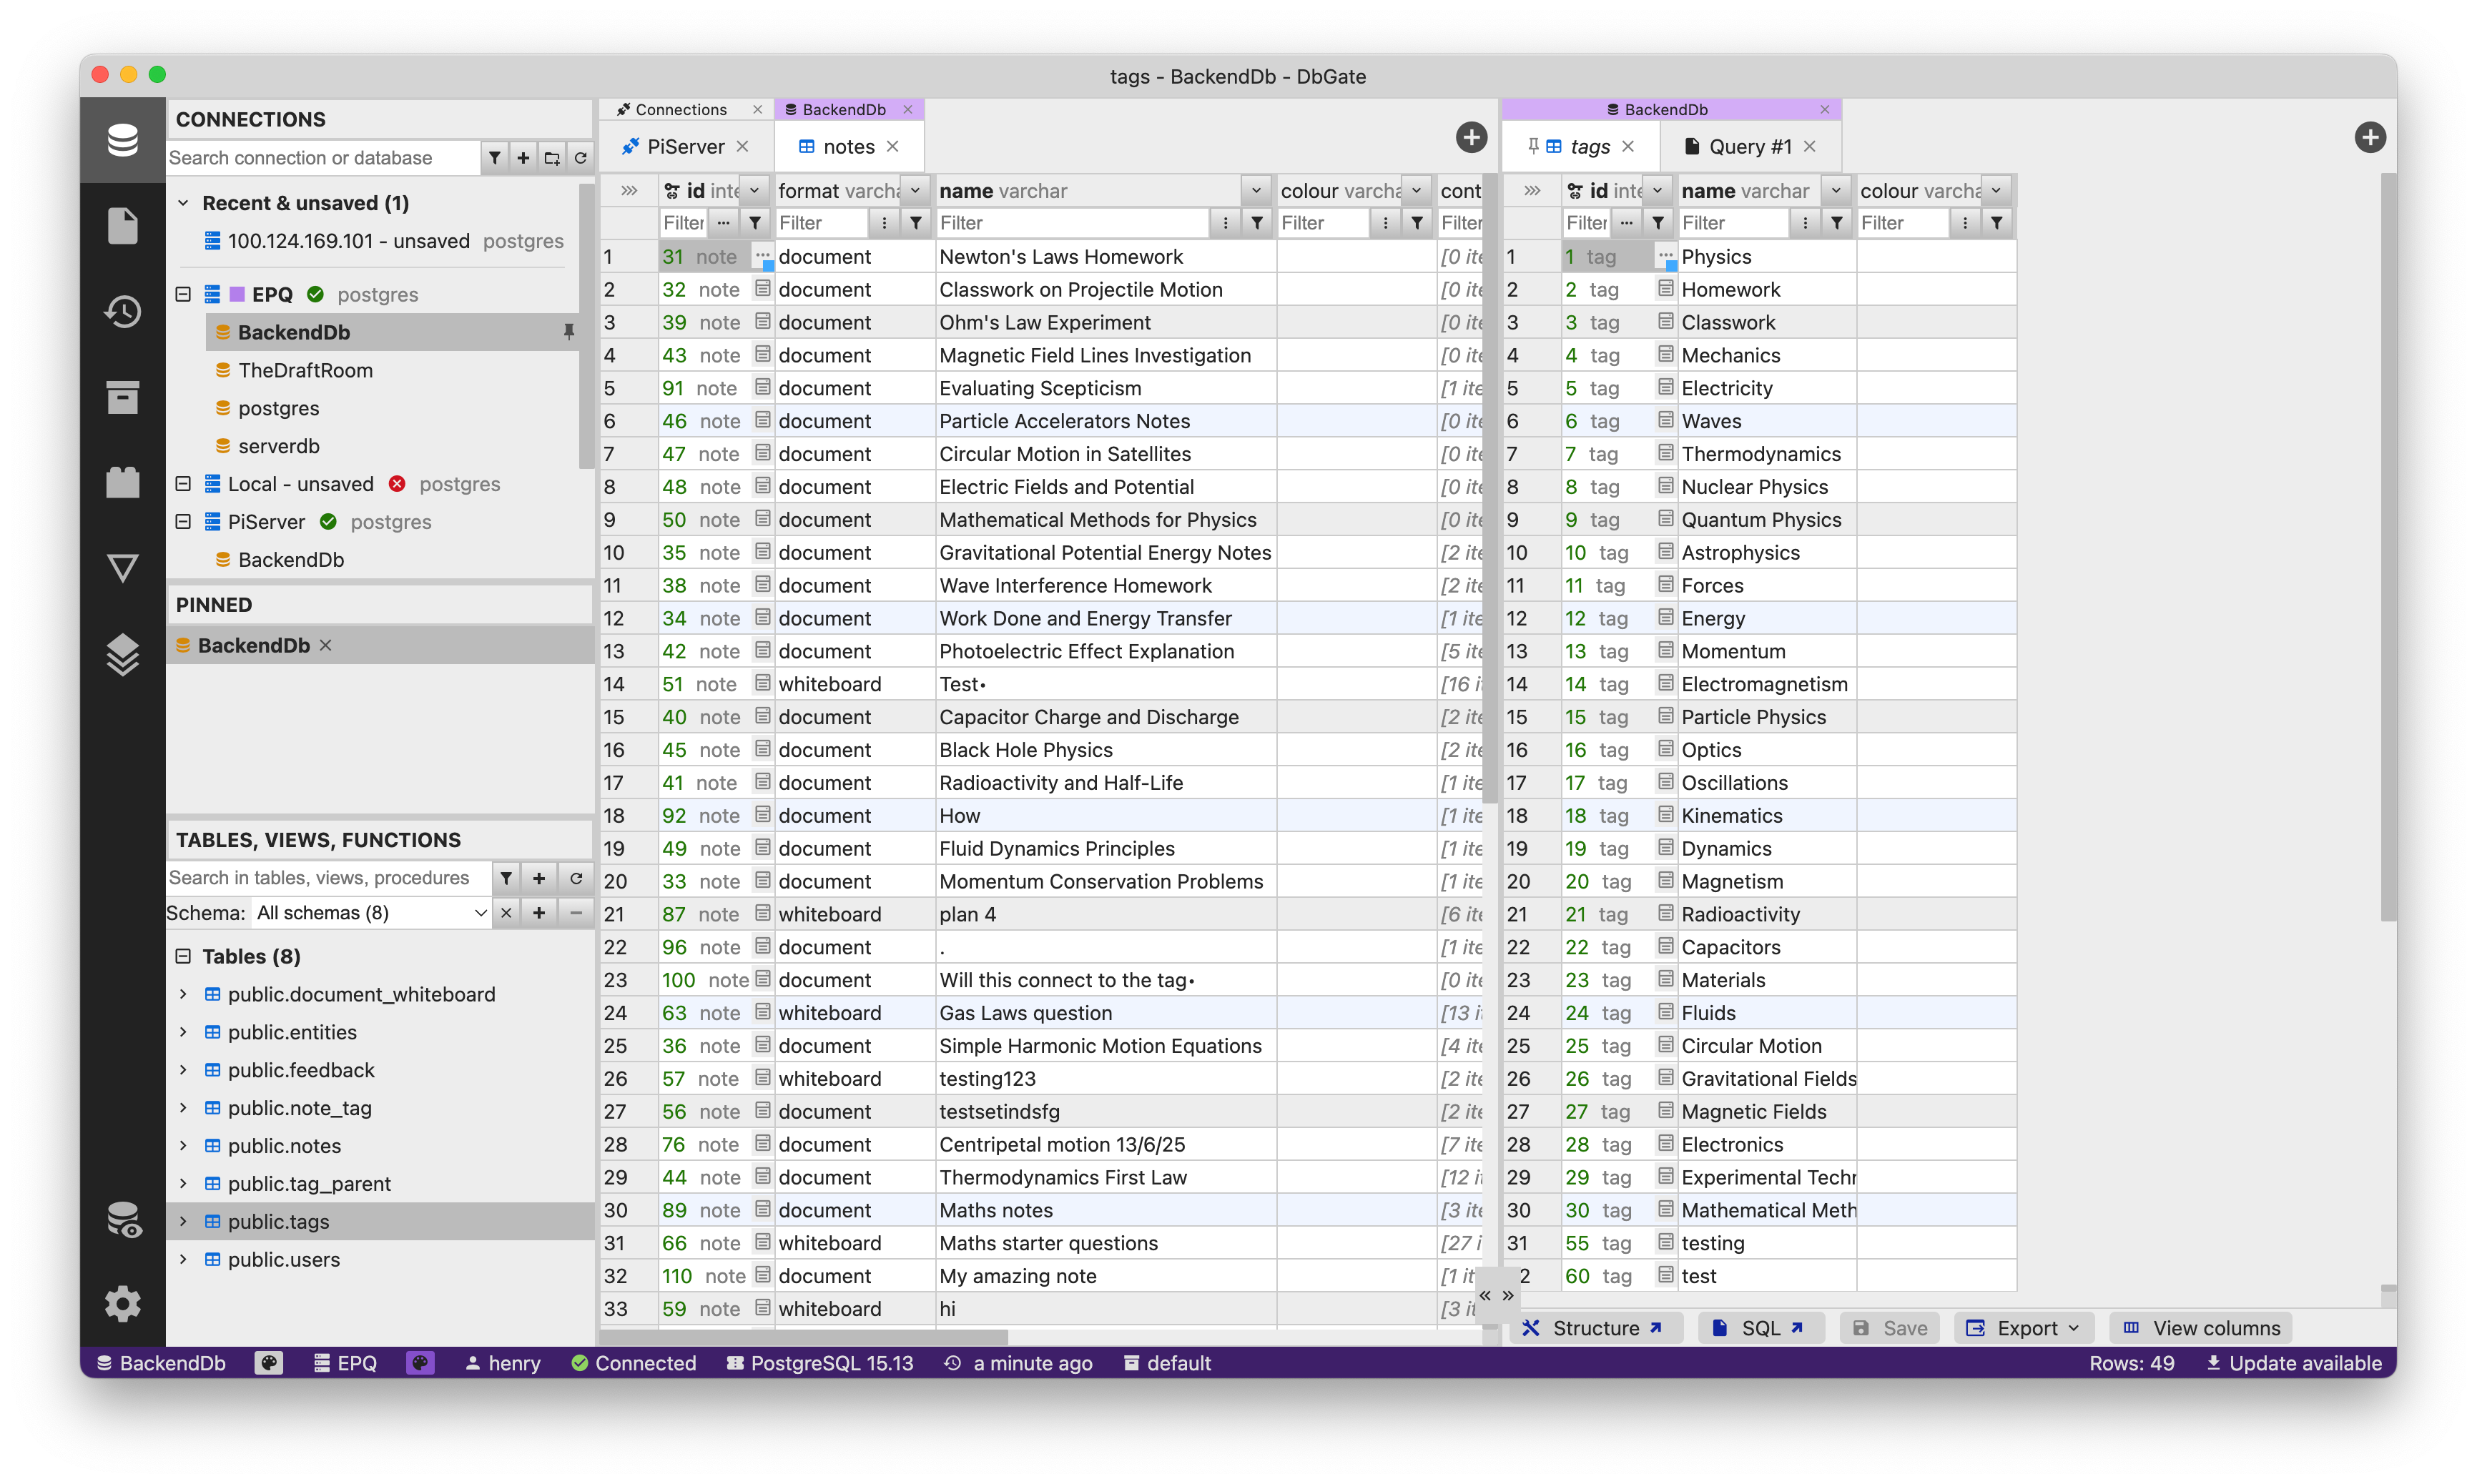
\includegraphics[width=0.8\textwidth]{SkillDevelopment/SkillsReflection/media/postgres.png}
    \caption{Connected to my Postgres database using dbGate}
\end{figure}

\subsection{Version Control:}
Version control was a skill I had heard about but never seriously applied before this project. I decided early on to use Git and GitHub to manage my code, which quickly proved invaluable. It allowed me to experiment with features without worrying about breaking the entire project and gave me a clear history of my progress over time.

Learning Git commands and workflows was initially daunting, but over time I became comfortable with staging, branching, and merging. Using version control also gave me a taste of professional software development practices, which strengthened the authenticity of my project. By the end, I realised that Git was not only a technical tool but also a mindset: a way of thinking about code as something collaborative, iterative, and constantly evolving.

Once I had mastered the basics of Git, I explored more advanced features such as pull requests and issue tracking. These tools helped me organise my work and plan future development tasks. Overall, version control transformed how I approached coding, making it more structured and manageable. 

\begin{figure}[H]
    \centering
    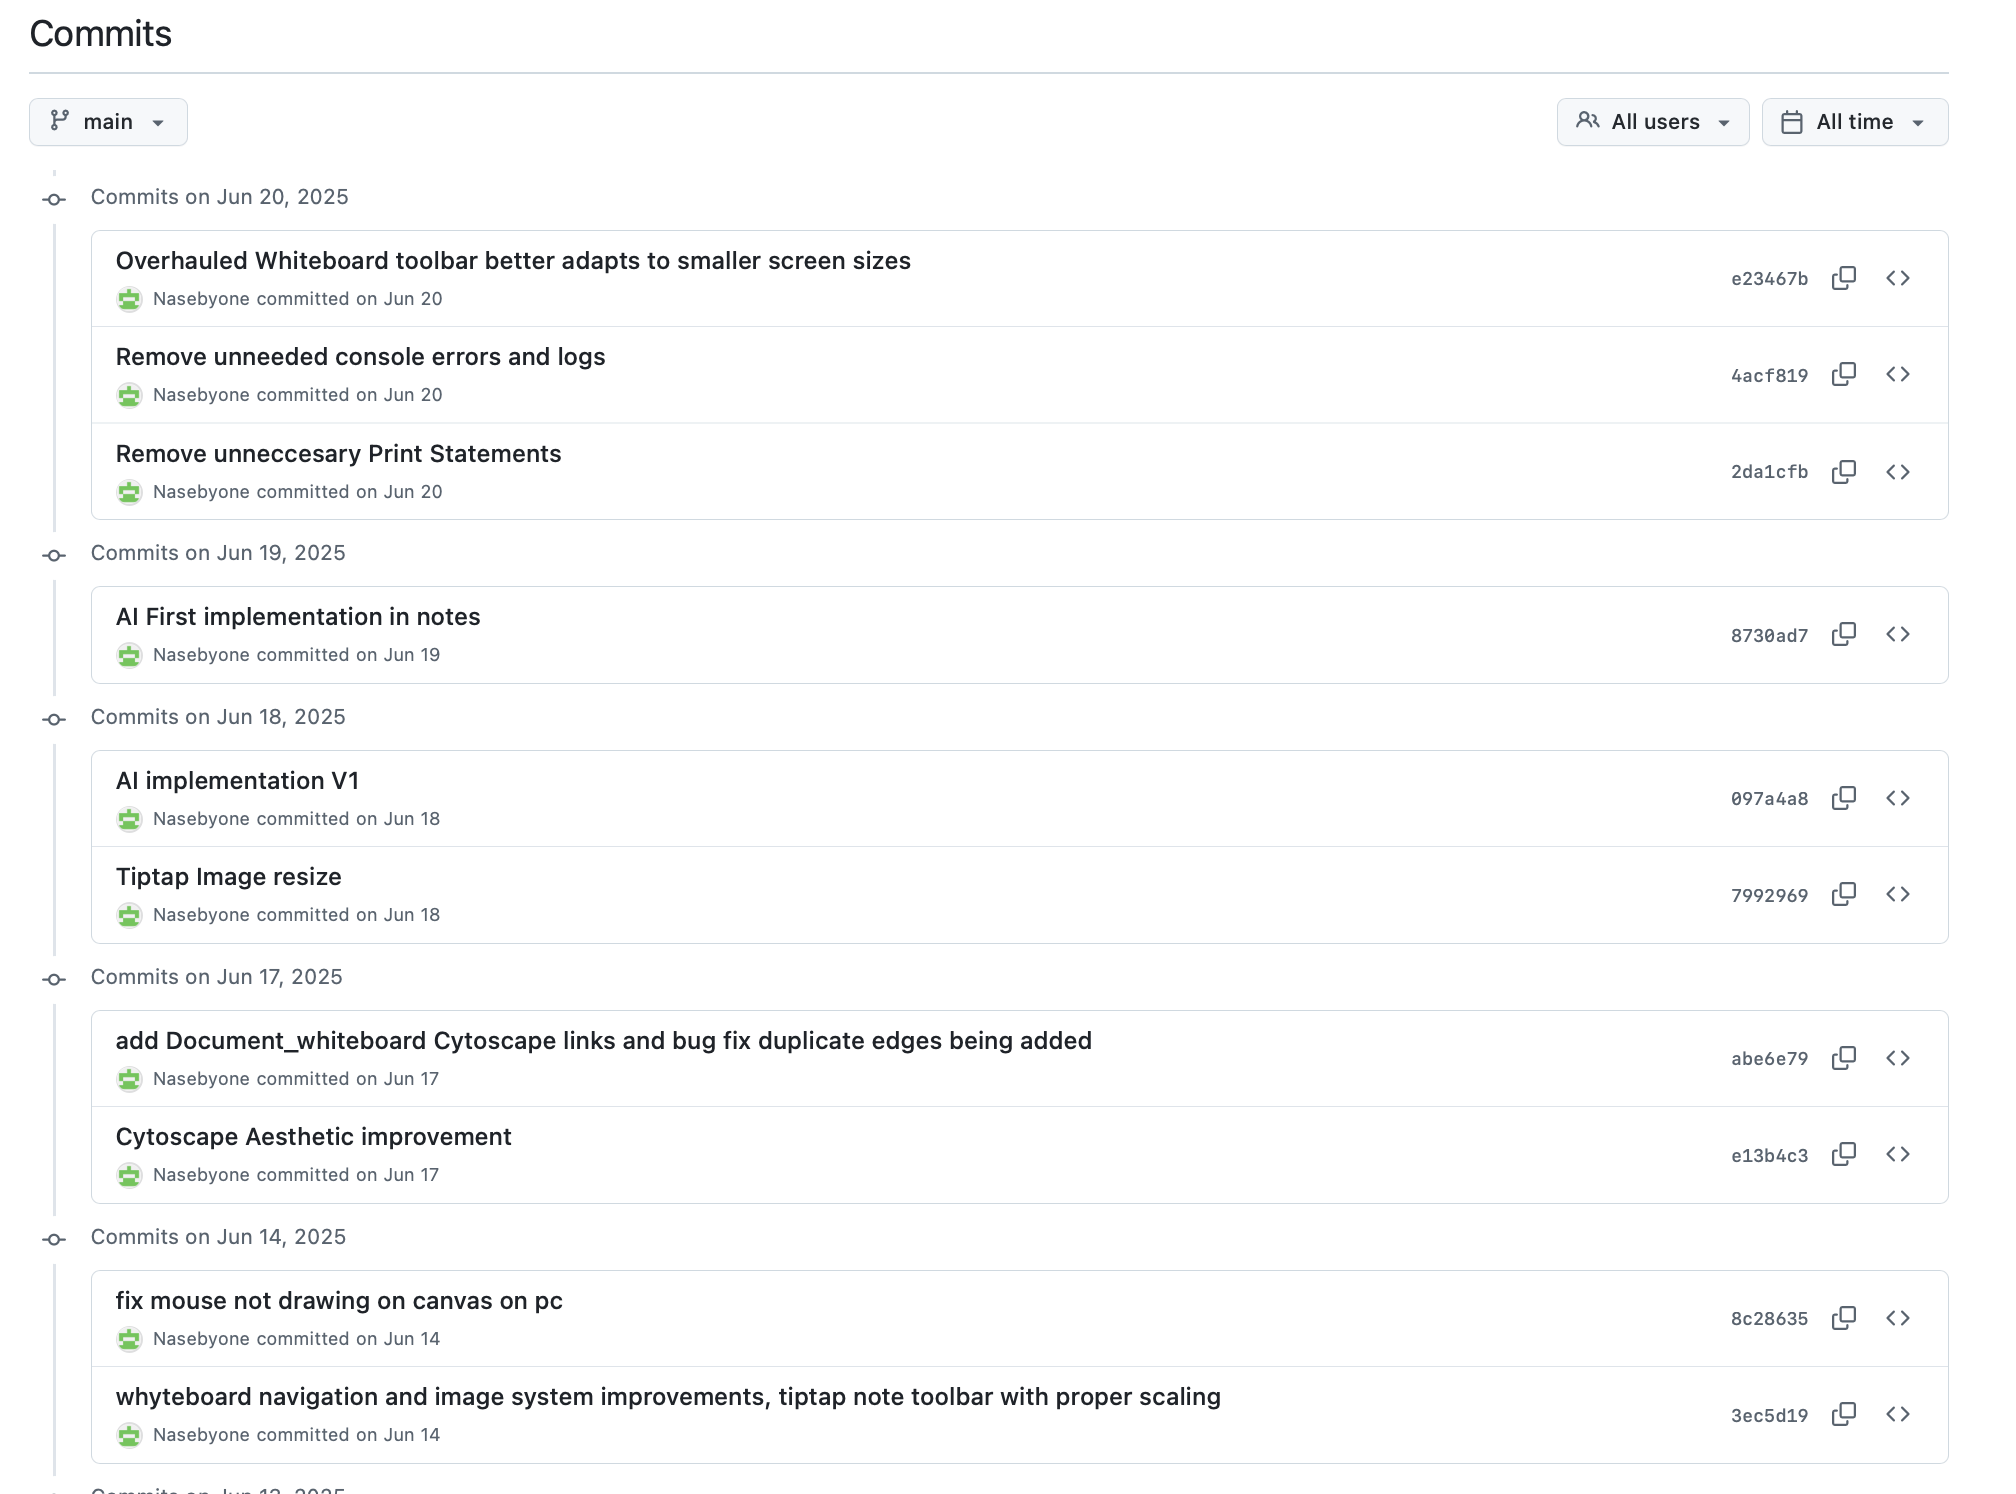
\includegraphics[width=0.8\textwidth]{SkillDevelopment/SkillsReflection/media/gitCommits.png}
    \caption{A snapshot of my GitHub commit history showing regular updates to my project}
\end{figure}

\subsection{Backend API Creation:}
One of the most technically demanding parts of my project was learning how to create and work with backend APIs. While frontend development focuses on what the user sees, the backend is what powers functionality behind the scenes. For NeuroNote, this meant creating systems that could securely handle note storage, user authentication, and data retrieval. I chose to use Python Flask because of its wide user base and excellent documentation, but I still needed to understand how API calls worked and how data flowed between client and server.

At first, I found it difficult to understand error messages and asynchronous code, but by breaking problems into smaller pieces and carefully reading documentation, I built up my confidence. Designing an API that could respond quickly and reliably taught me a lot about scalability and user expectations. Looking back, I feel this skill pushed me far outside my comfort zone as it required thinking about problems in a new, high level way, but ultimately gave me one of the most valuable technical experiences of the whole project.

\subsection{Digital Content Hosting:}
Hosting the project online was another steep learning curve. Until now, most of my coding projects had been confined to my laptop, but with NeuroNote I wanted a live, accessible product. This meant setting up hosting and learning about domains, DNS, and deployment pipelines. I registered the domain Neuronote.space, which gave the project a professional identity, began researching options to make my code public.

My main constant here was budget, ideally i wanted to spend as close to £0 as possible. Whilst financial limitations can often disadvantage software companies, i found it to be the opposite here. I was forced to think creatively and find free or low-cost solutions that still met my needs. After researching various platforms, I decided to use Cloudflare to open my Raspberry Pi to the internet, and I used a combination of free open source projects to host my backend and frontend cod on the aforementioned Raspberry Pi.

The process taught me about the difference between local development and live environments, especially the importance of testing in both. I also learned how to handle updates without disrupting users, and the satisfaction of seeing my work accessible from any device was a huge motivation. Hosting gave the project a sense of realism: it transformed it from a school task into something that felt tangible and “real-world.”


\begin{figure}[H]
    \centering
    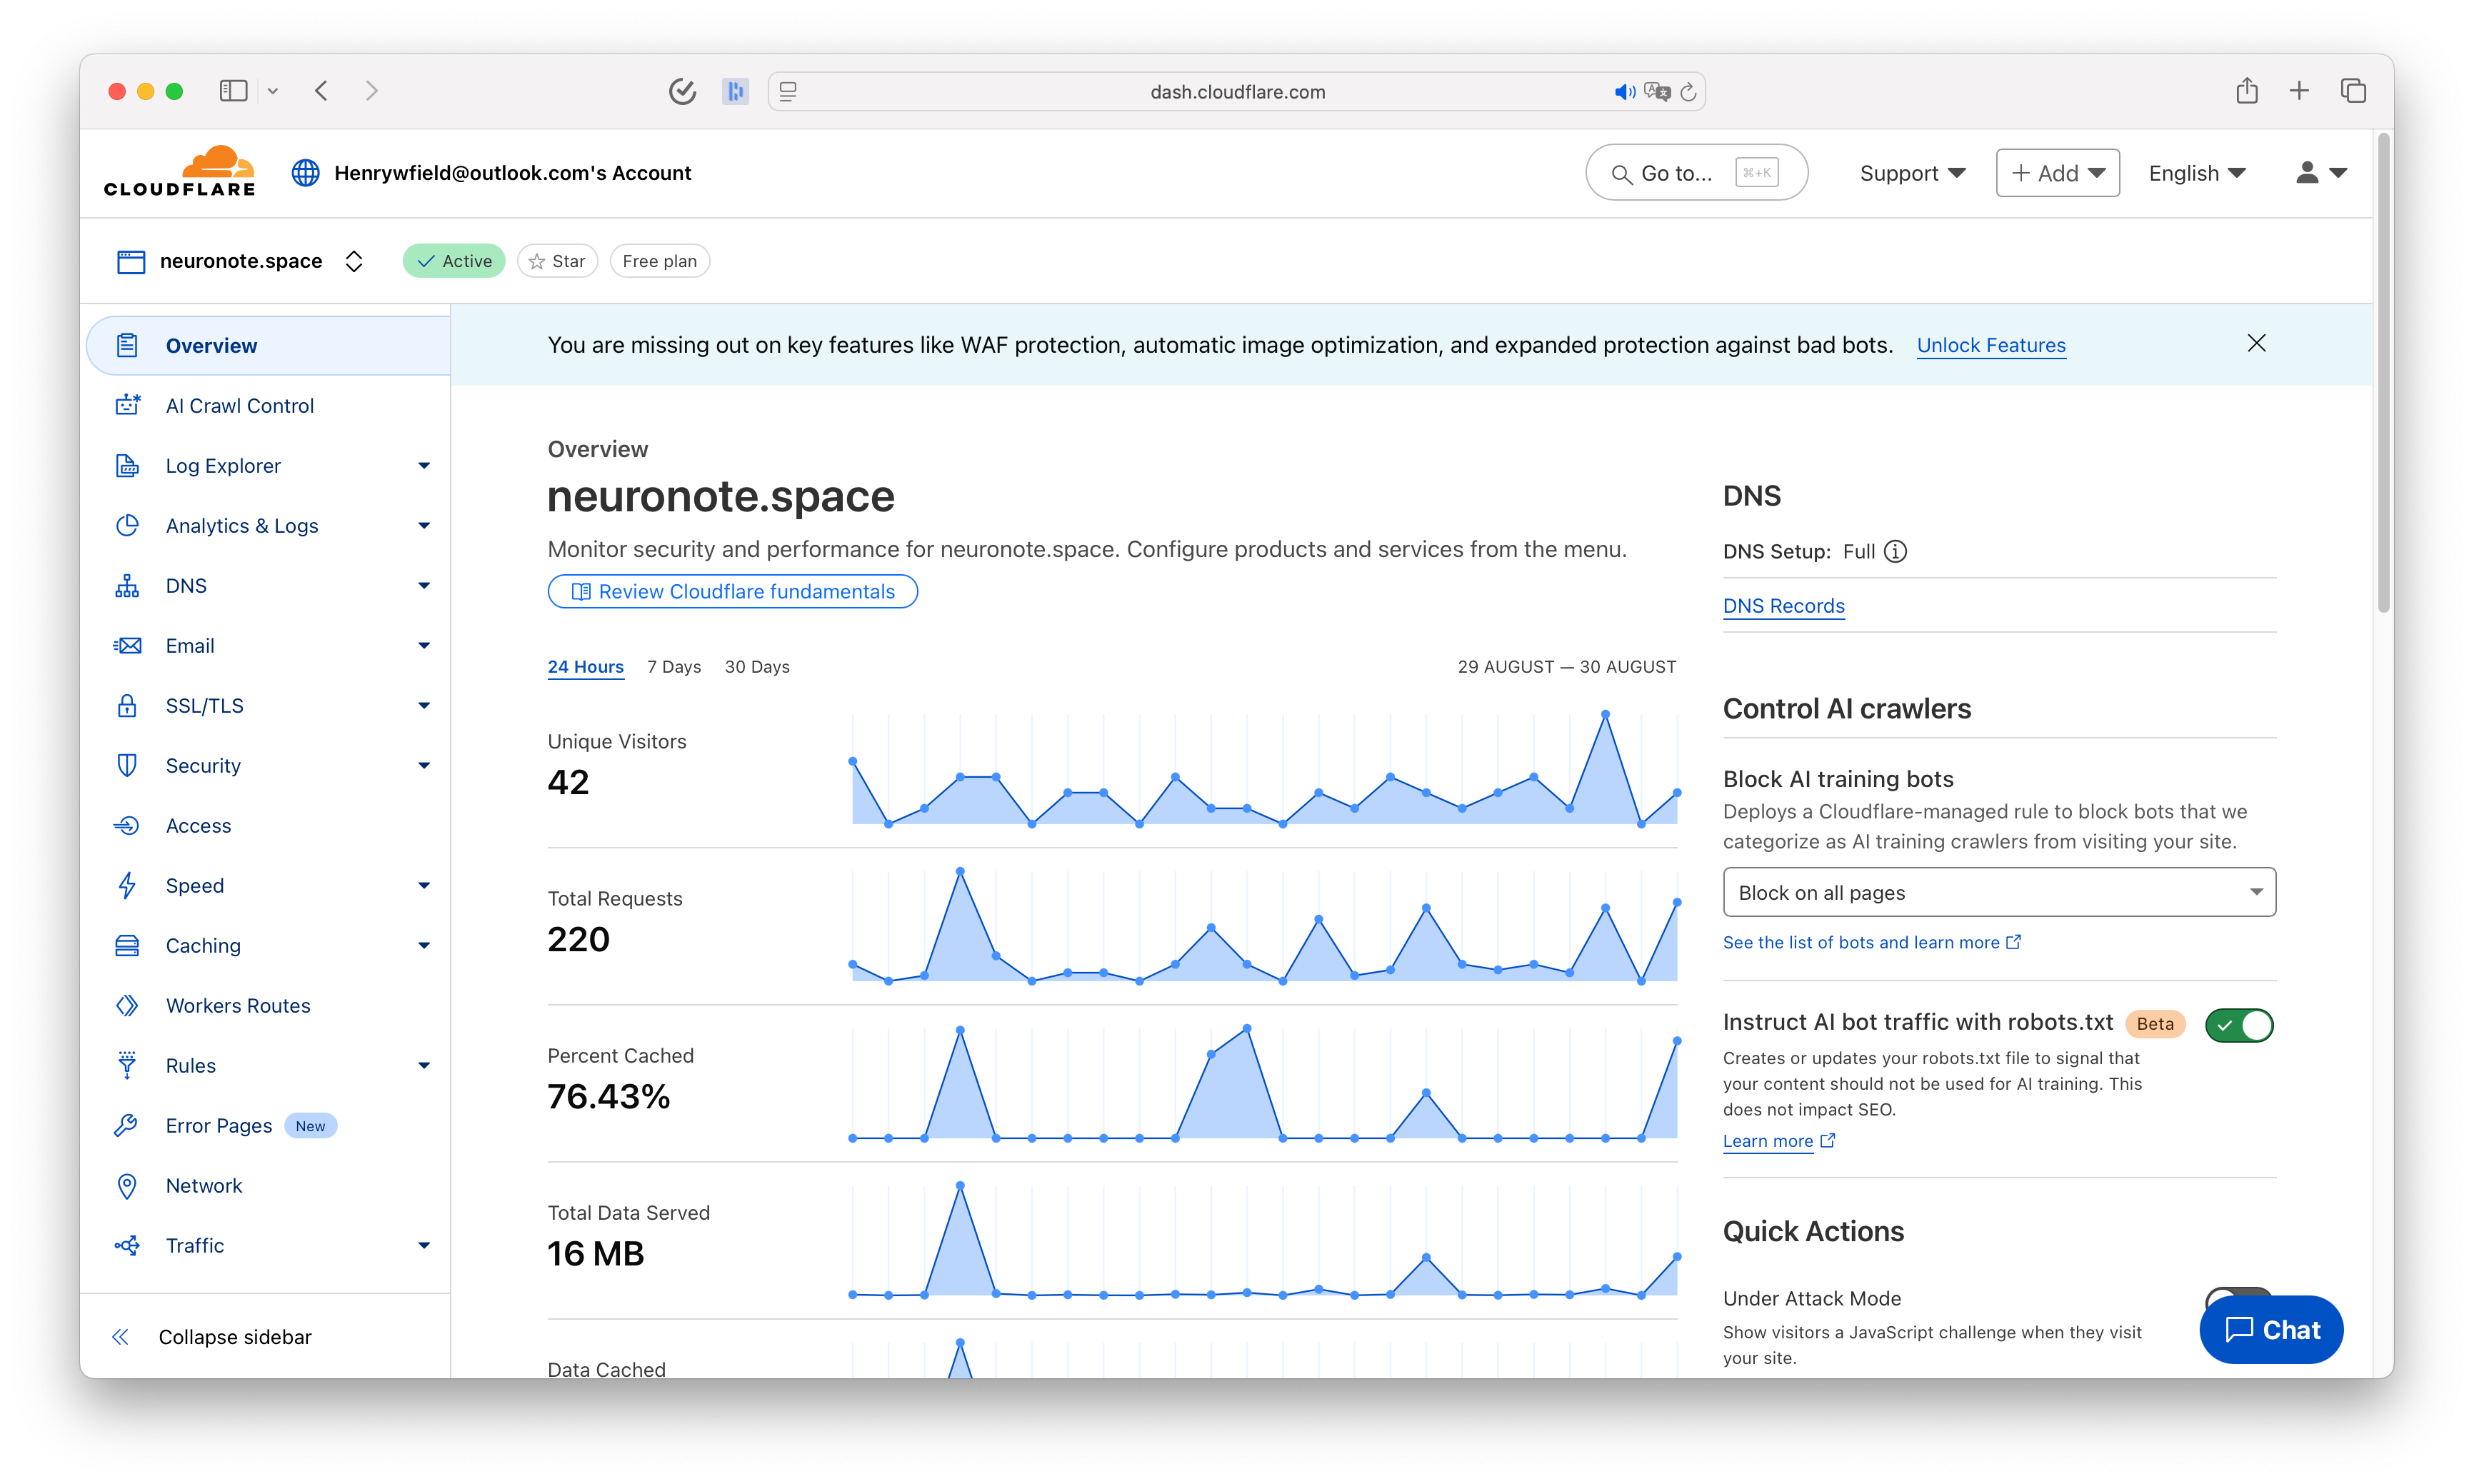
\includegraphics[width=0.8\textwidth]{SkillDevelopment/SkillsReflection/media/cloudflare.png}
    \caption{My Cloudflare dashboard where I can fully manage my domain and hosting}
\end{figure}

\subsection{Network \& Data Security:}
Working with user data meant that I had to consider security from the very beginning of my project. Even though NeuroNote was a prototype, I recognised the responsibility of handling information safely, especially if I wanted users to test the system with their own notes. Using robust JWT (JSON web token) authentication introduced me to secure login methods such as password hashing, which I researched in order to better understand the risks of insecure systems.

\begin{figure}[H]
    \centering
    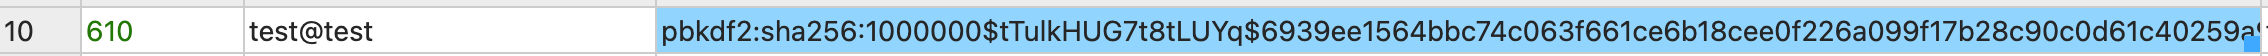
\includegraphics[width=0.8\textwidth]{SkillDevelopment/SkillsReflection/media/examplePassword.png}
    \caption{Example of a user's password which is safe to show as it is hashed and salted (encrypted)}
\end{figure}

I also became more aware of general security principles such as the importance of HTTPS, avoiding hardcoded keys, and limiting permissions where possible. Although I am far from an expert, this exposure to security concerns gave me a stronger foundation for thinking critically about software beyond functionality. It made me realise that a product is only as good as its ability to protect its users.

I should clarify that I made it clear to all users that this was a prototype and not suitable for sensitive data, but I still wanted to implement best practices wherever possible. This mindset of prioritising security will undoubtedly influence my future projects, as I now understand that protecting user data is a fundamental aspect of responsible software development.

\subsection{Market \& Existing Product Research:}
Early in the project, I knew I wanted to create a note-taking tool, but without research I risked reinventing the wheel or overlooking what already worked. I therefore dedicated time to analysing popular platforms such as Notion, Obsidian, OneNote, and Notability. I noted their strengths, such as Obsidian's plugin system and Notion's flexibility, but also weaknesses such as cluttered interfaces or steep learning curves.

This research not only guided my design but also helped me think strategically. I began to ask: “What makes people adopt one product over another?” and “How can I differentiate my tool while still meeting expectations?” These questions kept me grounded and ensured that I was addressing a real gap in the market. Without this research, my project might have been too narrow, but by engaging critically with competitors, I created something more focused and original.

\subsection{Primary Research:}
To balance my market research, I also conducted primary research with potential users. I started with surveys distributed among peers to gather their thoughts on existing note-taking tools, asking about pain points, preferences, and desired features. This gave me valuable data to back up design choices rather than relying only on my own perspective.

In addition, I shared early prototypes with small groups, asking them to test the application and provide feedback. Observing how others used my tool was eye-opening - features I thought were obvious sometimes confused users, while seemingly small touches were highly appreciated. This iterative testing loop not only improved the product but also sharpened my ability to ask the right questions and interpret qualitative feedback effectively.


\subsection{Feedback Collection:}
Feedback became one of the most consistent and useful drivers of progress throughout my EPQ. At first, I felt nervous about sharing unfinished work, worried that criticism would discourage me. However, I quickly realised that early and frequent feedback was the fastest way to identify flaws and opportunities. I began to actively seek it out, whether through structured surveys, informal conversations, or posts online.

I also learned how to process feedback constructively. Not every comment could (or should) be implemented, so I developed the skill of filtering suggestions, identifying common themes, and prioritising what would bring the most benefit to the user base. By the end of the project, I had built up resilience and confidence, seeing feedback not as criticism but as collaboration.

Using feedback so frequently even resulted in me building my own feedback form within the application and wider feedback system, allowing users to submit thoughts directly from the interface with my tools categorising this data instantly for review. This not only streamlined the process but also reinforced the idea that user input was central to the project's success.
% FEEDBACK SYSTEM

\begin{figure}[H]
    \centering
    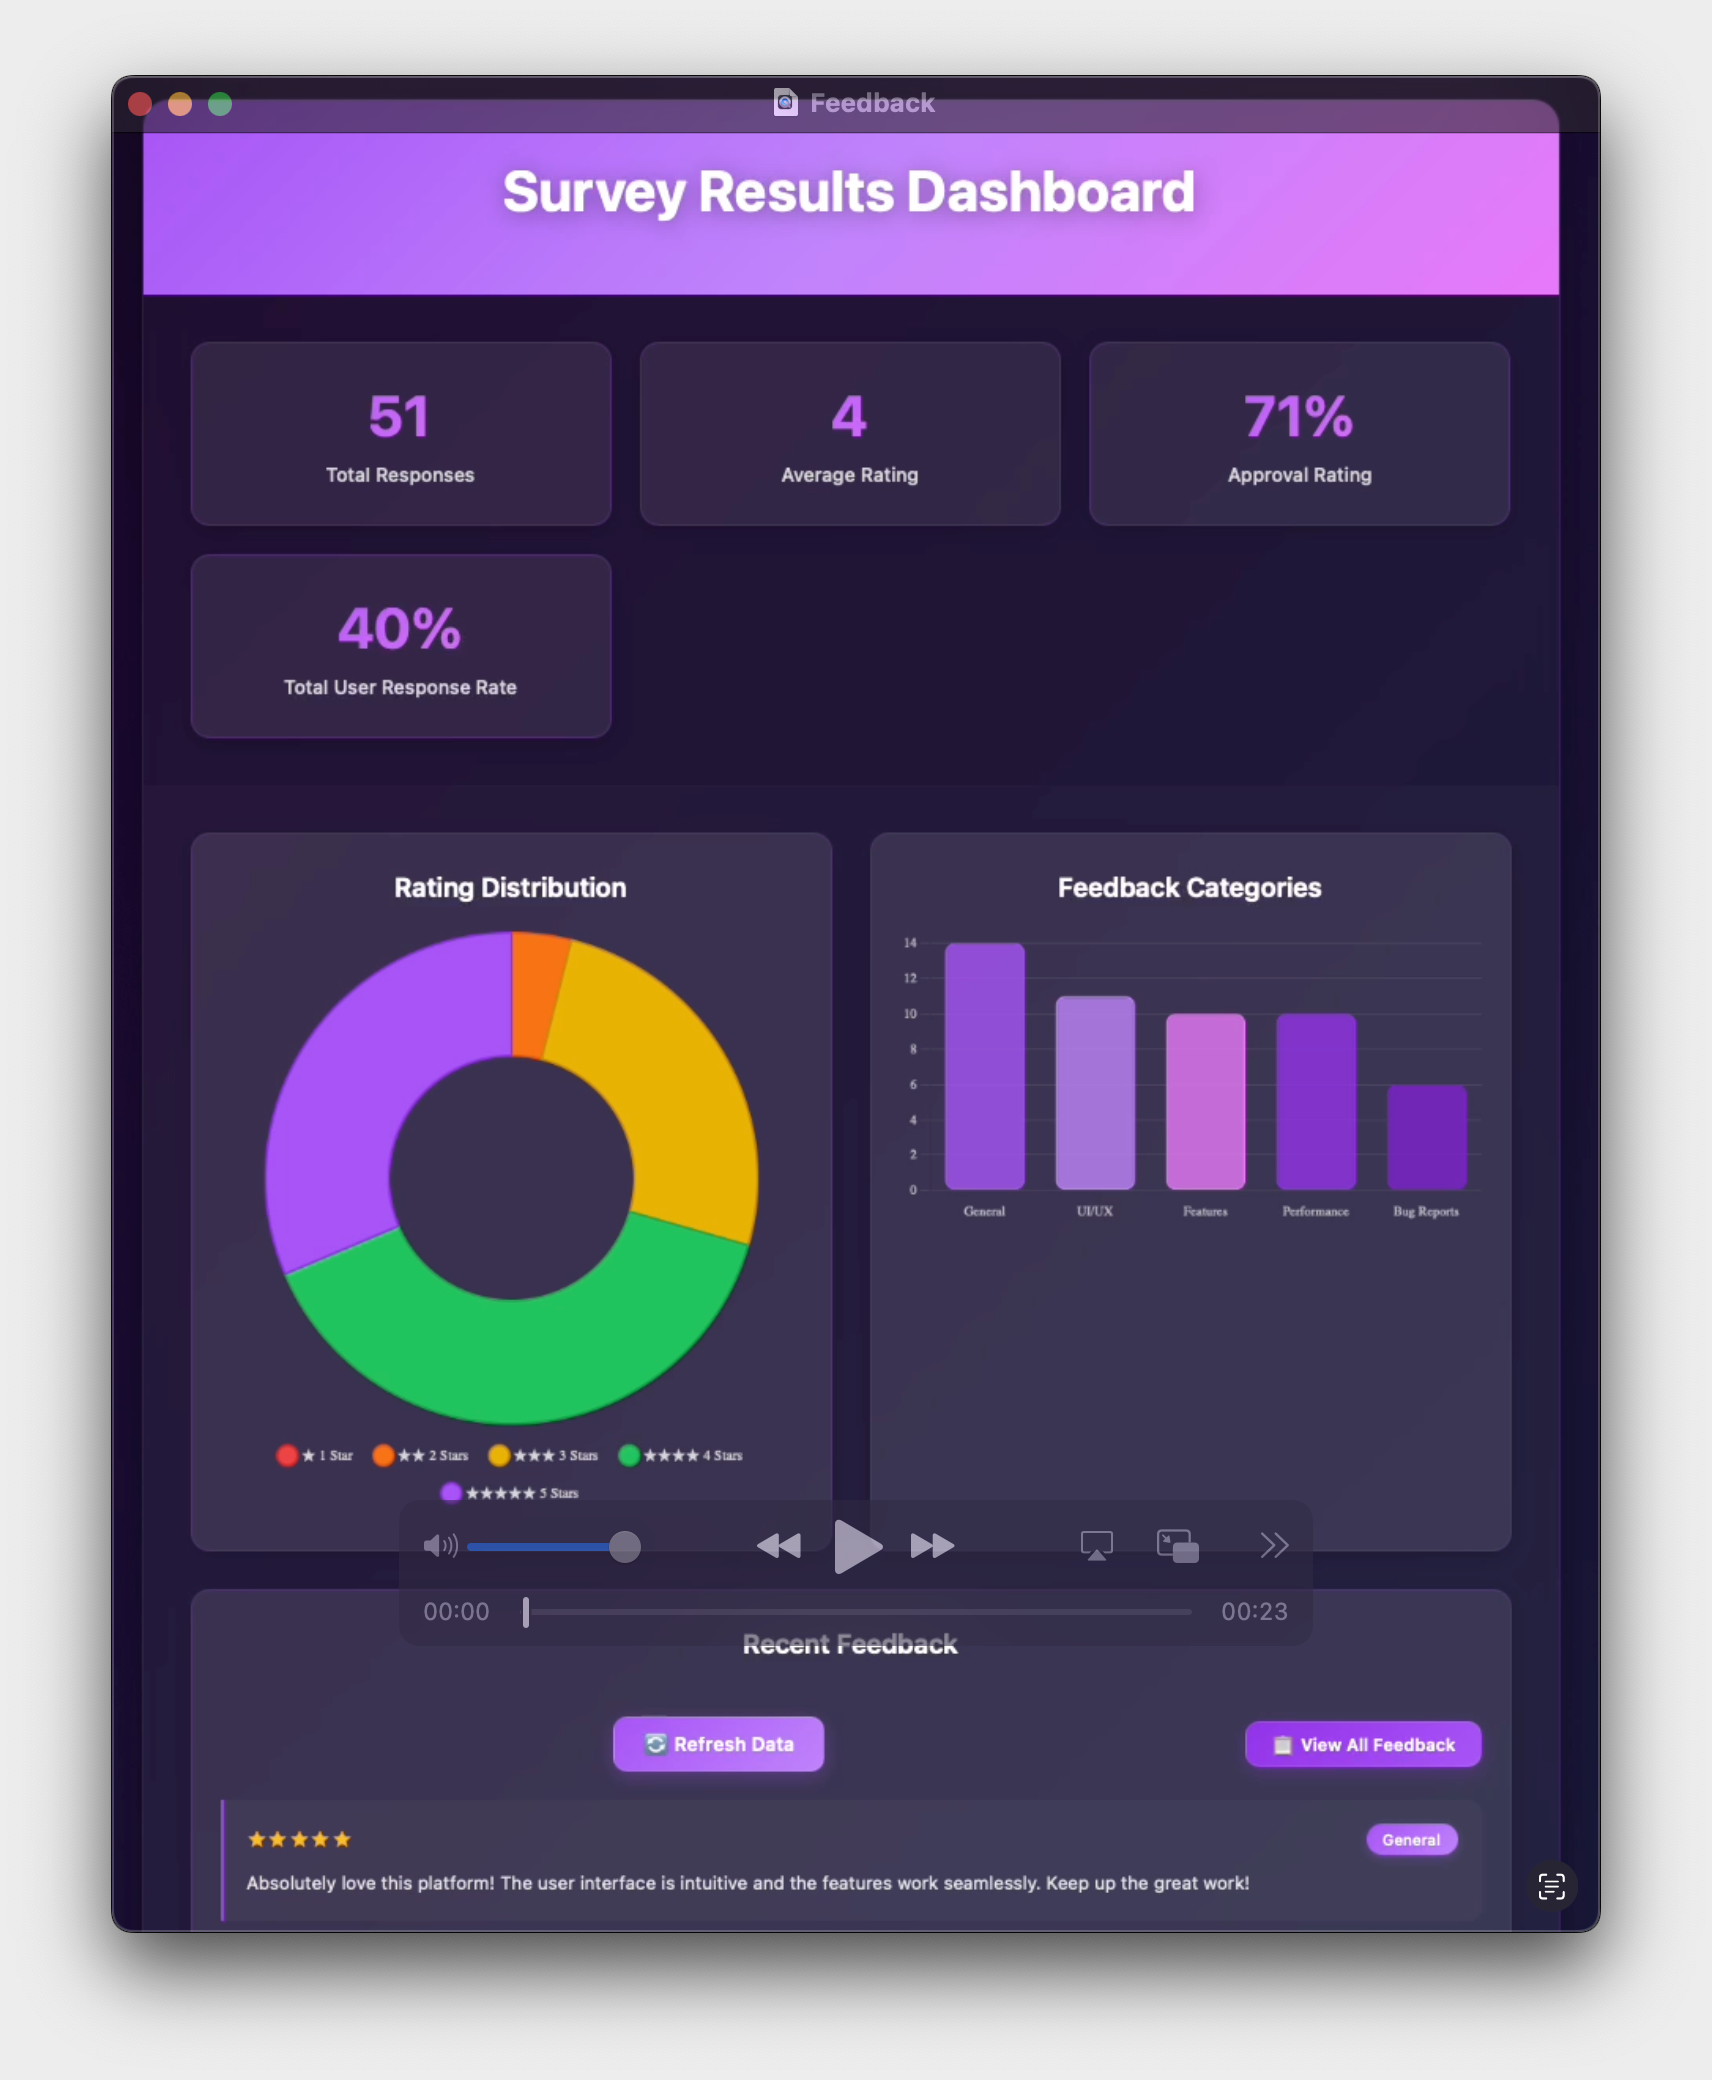
\includegraphics[width=0.4\textwidth]{SkillDevelopment/SkillsReflection/media/surveyApp.png}
    \caption{My custom feedback form's dashboard view for admins}
\end{figure}

\subsection{Self-Evaluation:}

Self-evaluation was an ongoing process during my EPQ, and I found that being reflective was just as important as being productive. I regularly paused to ask myself what was working, what wasn't, and how I could improve my approach. Sometimes this meant rethinking a technical choice, other times it meant adjusting my workflow or rebalancing time between software development and research.

Documenting this continual reflection in my Diary helped me become more honest about my strengths and weaknesses. Over time, I noticed patterns - for example, I tended to overestimate how quickly I could implement new features in the short term, but I was consistently strong at gathering and applying feedback. Recognising these tendencies allowed me to adapt and grow as a learner, which I believe was one of the most valuable outcomes of the whole project.

\subsection{Comparative analysis:}
Comparative analysis played a major role in both design and evaluation. By setting my work against industry leaders like Notion and Obsidian, I could see where I fell short but also where I had carved out unique value. This balance of humility and confidence was essential: I was not competing with billion-dollar companies, but I could still identify spaces where a simpler, more accessible tool might succeed.

I also compared different design iterations of my own work, analysing how small changes affected usability. This methodical approach prevented me from being too attached to one idea and reminded me that design is iterative. The skill of comparative analysis, weighing alternatives, identifying trade-offs, and choosing the best fit, is one I will continue to apply well beyond this project.

\subsection{Impact Analysis:}
 Even though NeuroNote is still a prototype, I reflected on how such a tool might influence students' learning habits if developed further. By combining note-taking with spatial and psychological principles, I believe it could help users engage more deeply with their material and potentially improve retention.

On a personal level, the impact was also significant. Working on this project taught me not only new technical skills but also professional habits that will benefit me in higher education and beyond. I gained a stronger understanding of how software can influence people's behaviour, which deepened my interest in pursuing computer science and psychology further. In this sense, the project's impact has already gone beyond the product itself, shaping my own development and ambitions.


\subsection{Market Analysis:}
Market Analysis was potentially one of the most important skills I have developed during my EPQ. At the start of my project I had a very vague idea of the market I was entering (and what it was I wanted to achieve). If I hadn't yet further explored the needs of my future potential user I could have spent 200+ hours developing software that was of no use to anyone other than myself. 

I found that frequent feedback collection and primary research conduction with a number of my peers was the most effective method to collect this valuable information. By initially sending out a survey about other peoples thoughts and opinions on the industry I began to understand not just the technical challenges I could overcome but also the workflow optimisations I could make. From here I utilised my frequent prototype iterations to send out a variety of software tests to gauge user response 



